\apendice{Especificación de diseño}

\section{Introducción}

En este apartado se van a documentar las decisiones de diseño más relevantes del proyecto, como el diseño de datos o el diseño de clases de algunos componentes del sistema. 

\section{Diseño de Datos}
Para el diseño de datos se ha decidido utilizar el modelo relacional debido a su similitud con los esquemas clave-valor que se utilizan en la base de datos basadas en documentos.


\subsection{DynamoDB}

Se ha utilizado la base de datos NOSQL basada en documentos DynamoDB.\\
La base de datos contiene 5 tablas, de las cuales 2 son versiones destinadas a ejecutar los tests / desarrollo. Cada uno de los elementos de la base de datos contiene dos atributos obligatorios, $updated\_at$ y $created\_at$, estos atributos son strings que almacenan una fecha en formato ISO 8601. 

\subsubsection{LudwigDataset}
Esta tabla contiene todos los items del conjunto de datos Ludwig \ref{fig:C:dynamo_dataset}. La clave primaria (o clave de partición en DynamoDB), se identifica como $PK$, y es un string que almacena el id de la canción en Spotify. Por otro lado, se almacena el $MBID$ de Brainz, un valor único en toda la tabla. Discogs \cite{C:a2022_discogs} tiene muchos más subgéneros que los listados en la memoria, por ello se almacenan el resto de subgéneros que no se van a utilizar para entrenar los clasificadores en el campo $otherSubgenres$. Los estados de ánimo almacenan un valor entre 0 y 1 que indican la confianza de ese estado de ánimo. 

La obtención de este dataset se realiza siguiendo el proceso indicado en el diagrama de la figura \ref{fig:ludwig_dataset}

\begin{figure}
    \centering
    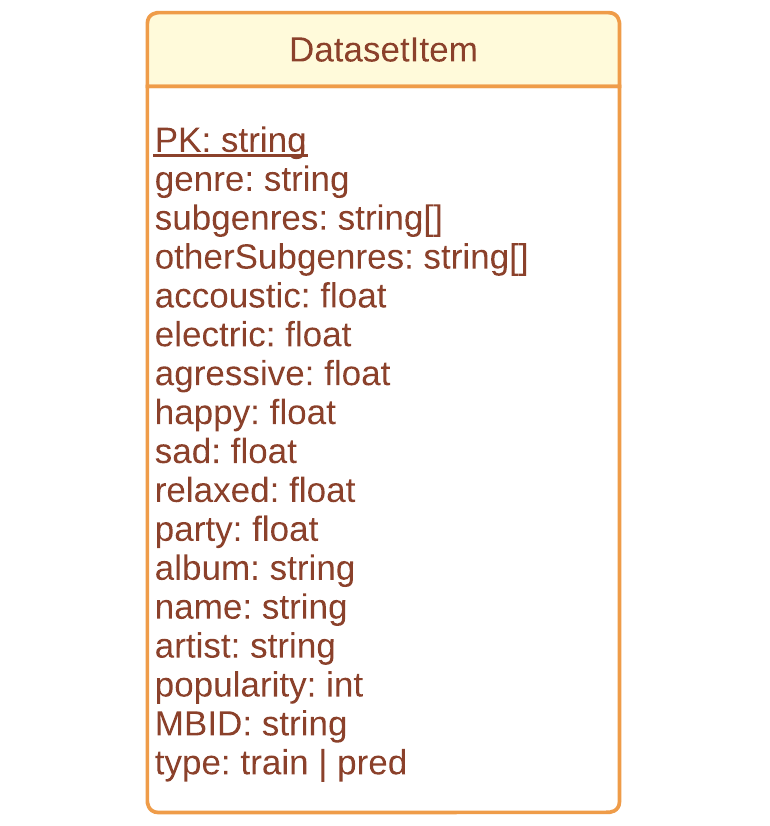
\includegraphics{img/C/data_dataset.png}
    \caption{DynamoDB: Ludwig Dataset}
    \label{fig:C:dynamo_dataset}
\end{figure}


\begin{figure}
    \centering
    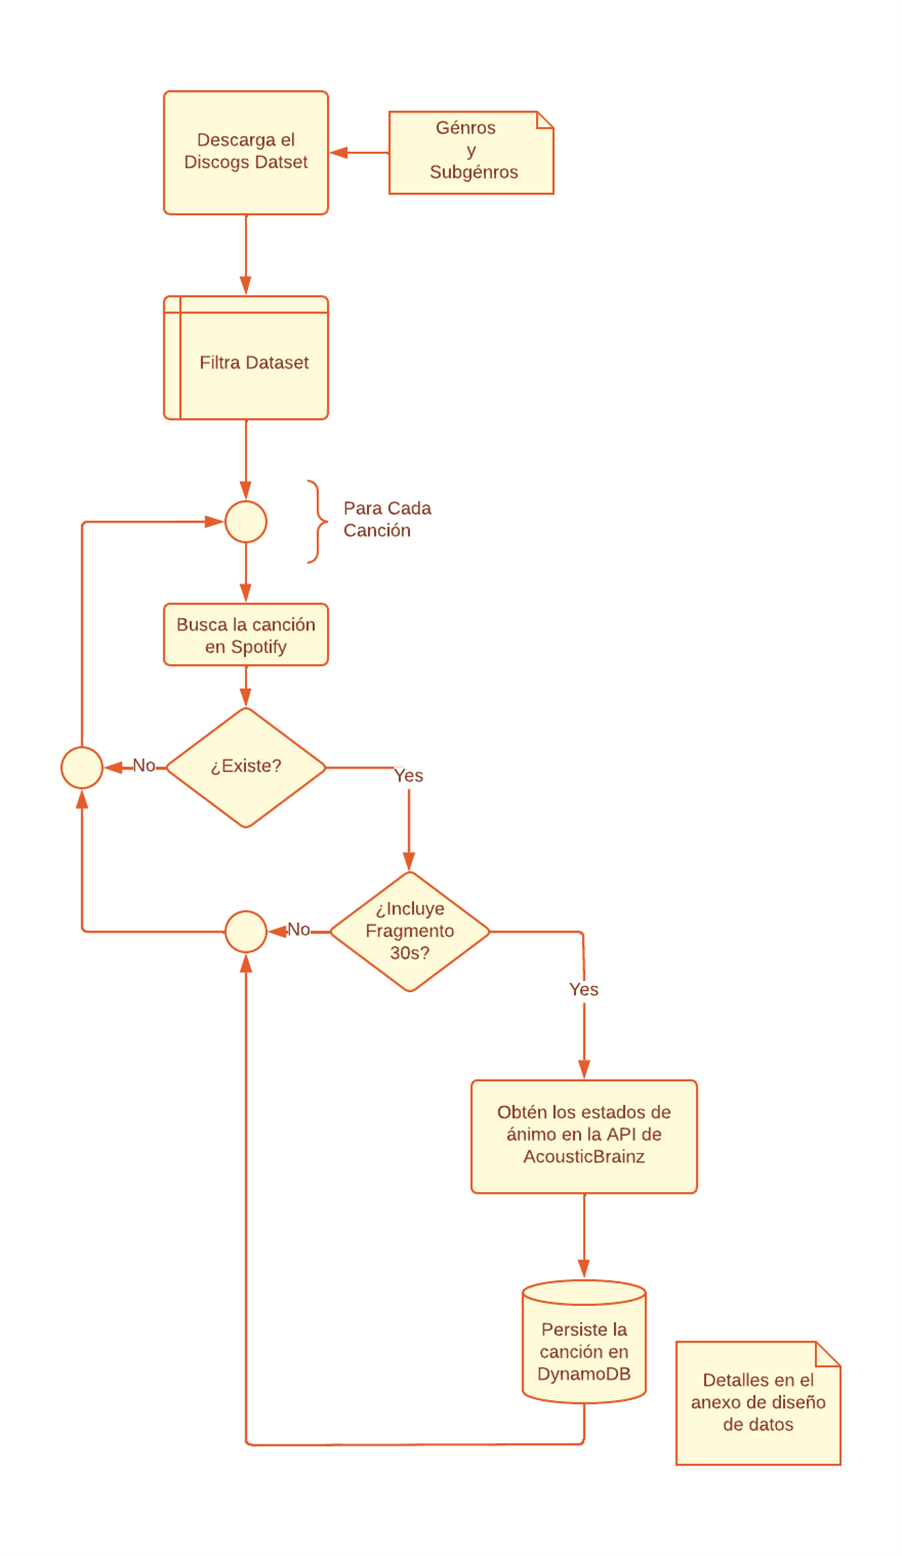
\includegraphics[width=12cm]{img/5/ludwig_dataset.png}
    \caption{Proceso de obtención de los datos de Ludwig Dataset}
    \label{fig:ludwig_dataset}
\end{figure}

\subsubsection{Tracks y Tracks\_test}
La tabla Tracks \ref{fig:C:dynamo_results} contiene los resultados del clasificador de géneros. \\
El identificador de la tabla, $PK$, almacena el id de Spotify de una canción. Esta tabla contiene un atributo $version$, que permite identificar la versión del clasificador, ya que si reemplazamos el modelo principal, es posible los resultados almacenados y los resultados del clasificador sean distintos.
La implementación de SpotMyFM obliga a DynamoDB a indexar $version$ para que únicamente se puedan obtener los resultados de la versión actual del clasificador.

\begin{figure}
    \centering
    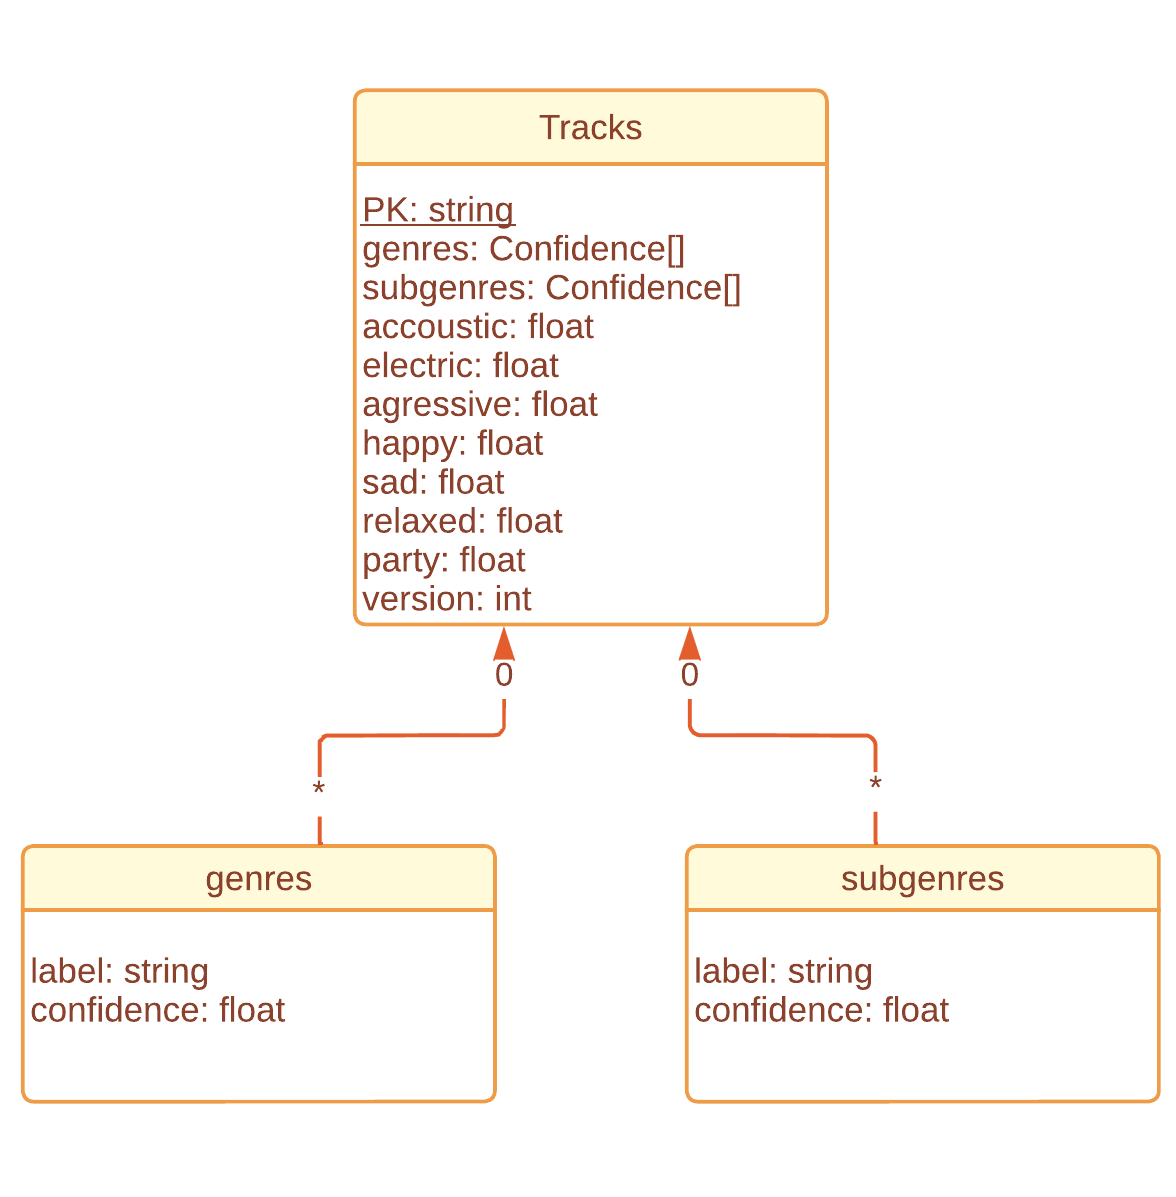
\includegraphics{img/C/data_tracks.png}
    \caption{DynamoDB: Resultados del analizador de canciones}
    \label{fig:C:dynamo_results}
\end{figure}

\subsubsection{Users y Users\_test}
La tabla Users \ref{fig:C:dynamo_users} contiene la información de los usuarios que han utilizado la función de etiquetas de SpotMyFM. Debido a la limitación de DynamoDB de 40kB por cada atributo, debemos almacenar las etiquetas asociadas a cada álbum mediante atributos dinámicos. Estos campos no se pueden declarar en Dynamoose, por lo que si queremos identificar que un campo es de un tipo específico, es necesario asignarle un prefijo, como por el ejemplo $ALB:<id\_album>$, donde $<id\_album>$ hace referencia al ID de Spotify del álbum.
\begin{figure}[]
    \centering
    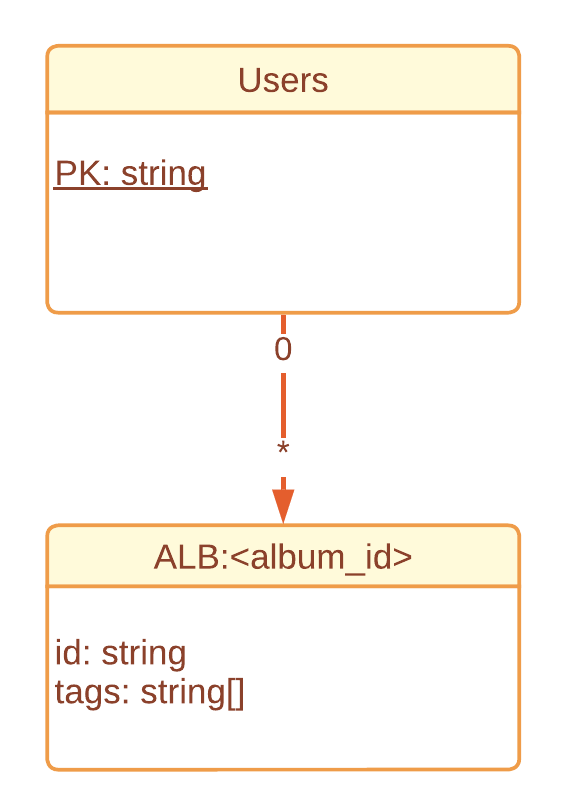
\includegraphics{img/C/data_users.png}
    \caption{DynamoDB: Tabla usuarios}
    \label{fig:C:dynamo_users}
\end{figure}

\clearpage

\subsection{Datos del Frontend} \label{C:datos_front}

Una de las fuentes de datos de la capa \textbf{modelo} \ref{modelo_vista_presentador} es DexieDB \ref{fig:c:dexie}, una base de datos NOSQL que utilizamos como caché intermedia para almacenar los datos obtenidos de las distintas fuentes de datos. 

Se ha diseñado el siguiente esquema relacional \ref{fig:c:dexie} mediante interfaces de Typescript. En este caso una canción está compuesta por un único álbum y uno o más artistas. Cada álbum está compuesto por uno o más artistas.

\begin{figure}
    \centering
    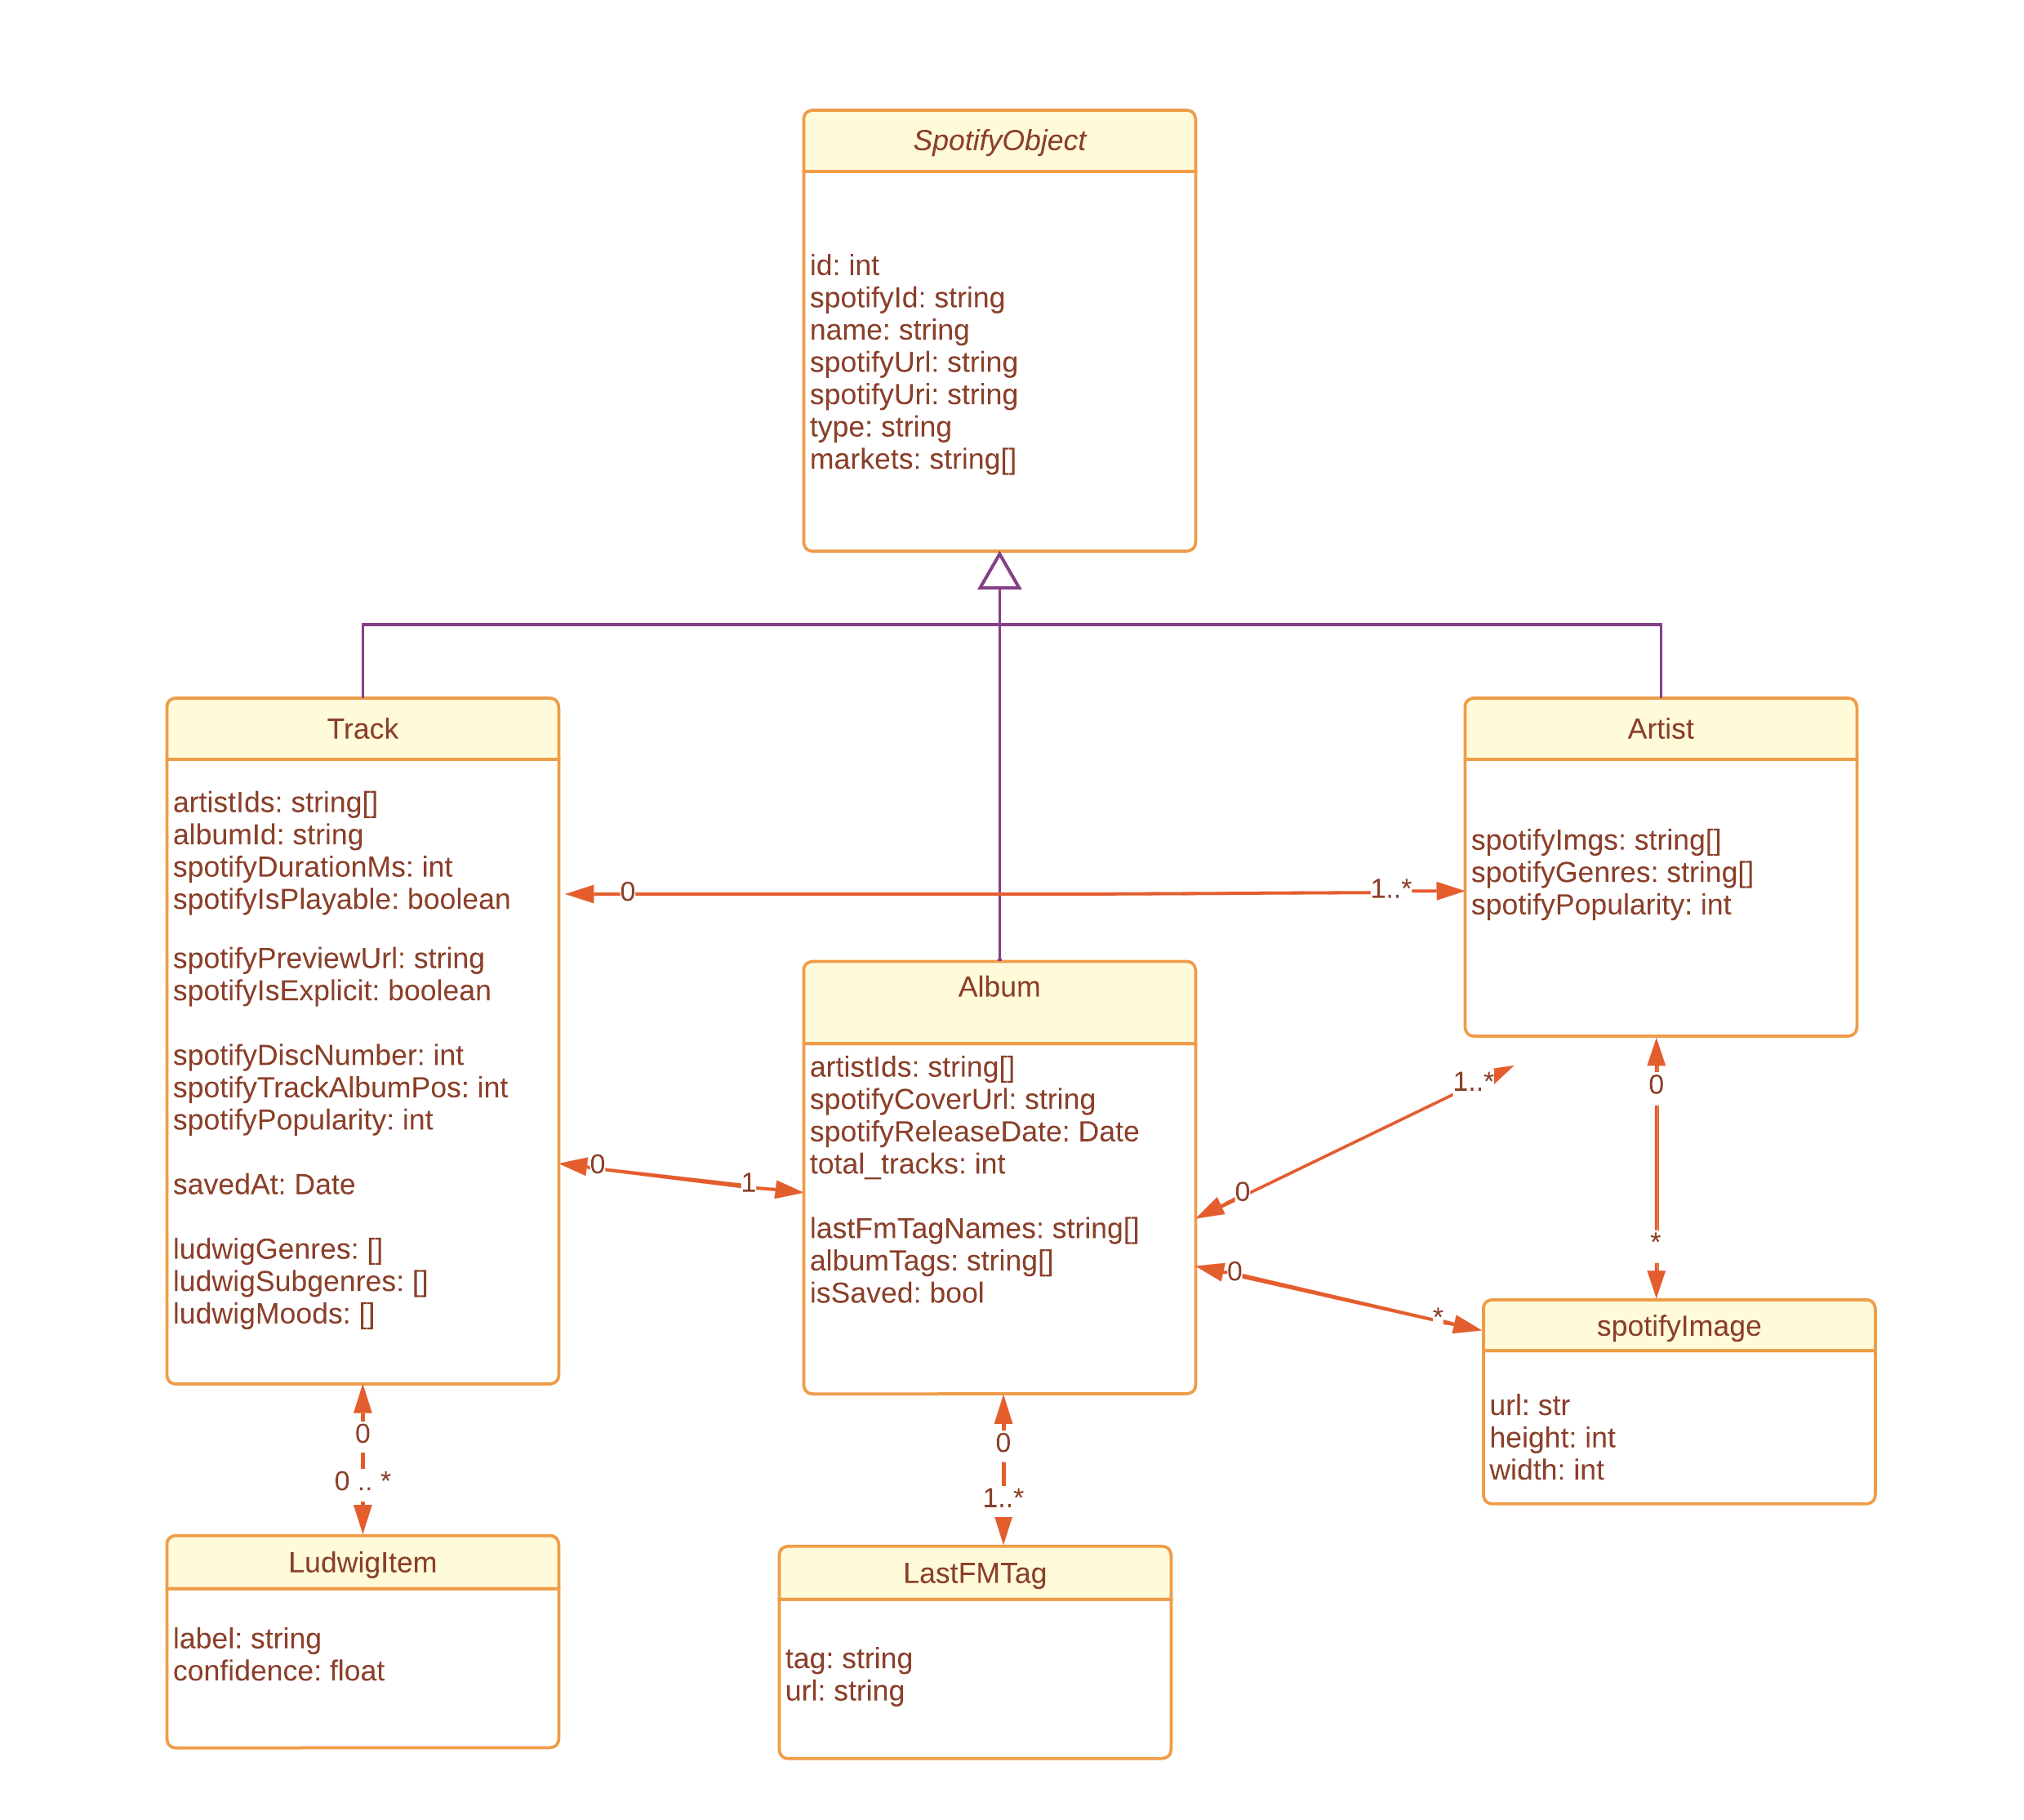
\includegraphics[width=\linewidth]{img/C/data_cache.png}
    \caption{DexieDB: Canciones, álbumes y artistas}
    \label{fig:c:dexie}
\end{figure}



\section{Diseño Procedimental}

Este apartado contiene el diseño detrás del inicio de sesión y la lógica de la fachada de datos \ref{C:fachada_datos}.



\subsection{Inicio de Sesión mediante Oauth2}

El inicio de sesión de Spotify utiliza el flujo de autenticación de Oauth2 \cite{oauth2}. En este flujo de identificación necesitamos dos claves, una pública y una privada.
La clave pública es accesible desde el frontend y sirve para identificar a la aplicación. La clave privada, gestionada desde el servidor web, permite verificar que un usuario desea utilizar nuestra API, y no se trata de un atacante intentando suplantar la identidad de la aplicación mediante la clave pública. 

\begin{figure}
    \centering
    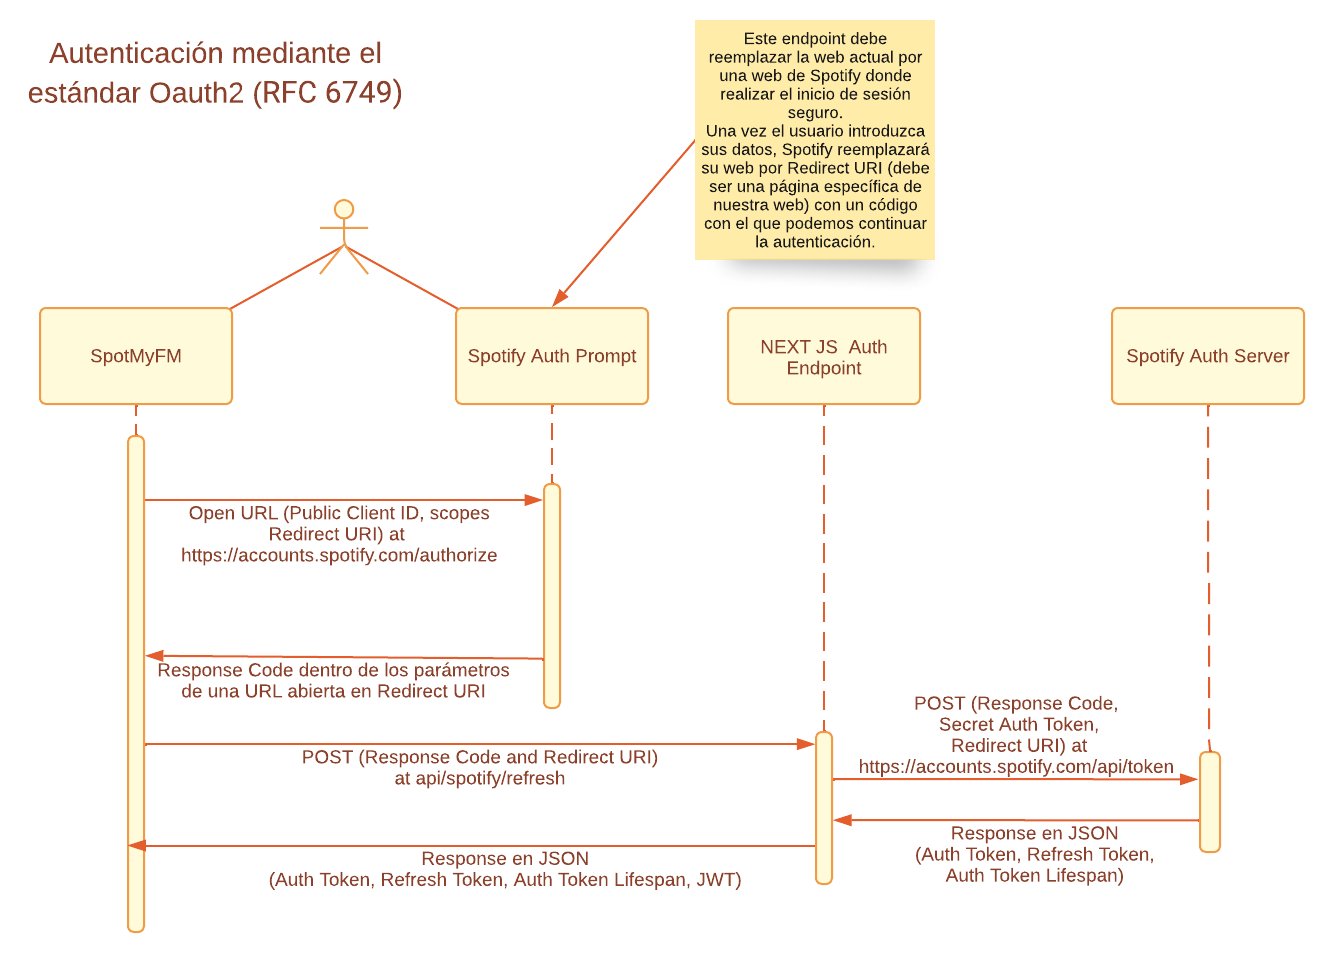
\includegraphics{img/C/oauth2.png}
    \caption{Flujo de Autenticación OAUTH2}
    \label{fig:oauth2_flow}
\end{figure}

En este flujo de autenticación \ref{fig:oauth2_flow}, el usuario abre una URL especial con el token público en los parámetros de la URL. Este token permite a Spotify identificar la aplicación, mostrando al usuario el nombre de la aplicación y los permisos que tiene que otorgar a la aplicación.\footnote{Estos permisos son conocidos en el estándar OAUTH2 como Scopes. }

Si el usuario acepta los permisos, Spotify abrirá una nueva pestaña con un segundo token de verificación en los parámetros de la URL. Este nuevo token se enviará al servidor web, donde se juntará con el token secreto para generar dos nuevos tokenes: un \textbf{token de autenticación} y un \textbf{token de refresco}. El token de autenticación permite al usuario interactuar con la API durante 1h, y el token de refresco permite generar nuevos tokenes de autenticación de 1h para que el usuario no tenga que iniciar sesión cada vez que pase 1h de uso.

En este paso aprovechamos a generar un token JWT con una vida útil de 1h con el siguiente contenido:

\begin{itemize}
    \item Token de Autenticación.
    \item Nombre de usuario.
    \item Identificador interno de Spotify.
    \item Booleano que indica si el usuario está suscrito a Spotify Premium.
\end{itemize}

Hecho estos devolvemos los 3 Tokens al frontend, donde se almacenarán en varias cookies para que sean accesibles entre sesiones. 

Para facilitar la gestión del flujo OAUTH2, se han diseñado dos clases \ref{fig:oauth_class} compatibles con el procedimiento que realizan esta tarea.

\begin{figure}
    \centering
    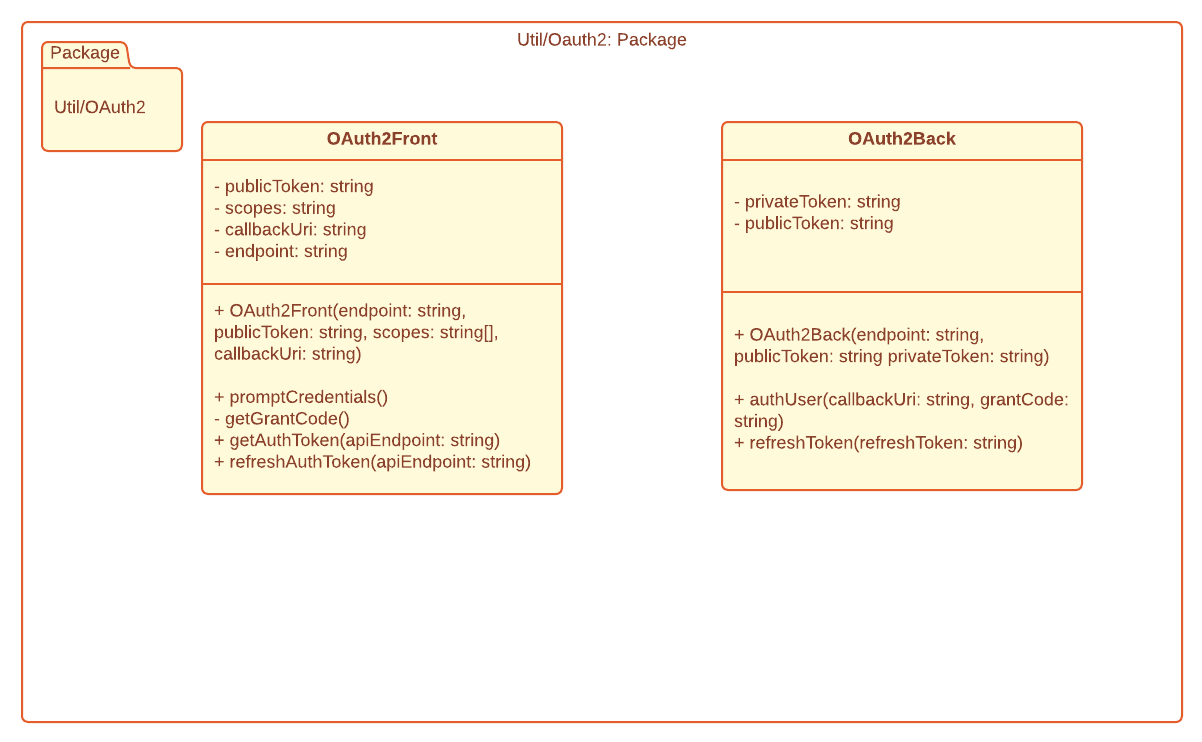
\includegraphics{img/C/oauth2_class_diag.png}
    \caption{Clases auxiliares para el flujo Oauth2}
    \label{fig:oauth_class}
\end{figure}

\subsection{Obtención de los Datos}\label{C:obtencion_datos_flow}

Uno de los objetivos de la fachada de datos \ref{C:fachada_datos} es unificar las distintas fuentes de datos para generar los objetos Fig.\ref{C:datos_front} con los que va a trabajar el presentador. Para ello se han planteado los siguientes diagramas de secuencia, que explican como obtener los datos de forma eficiente de cada una de las fuentes de datos. 

La figura \ref{fig:C:spotify_fetch} hace referencia a como se obtienen todas las canciones completas a partir de una lista de IDs realizando el menor número de peticiones posible. 

\begin{figure}
    \centering
    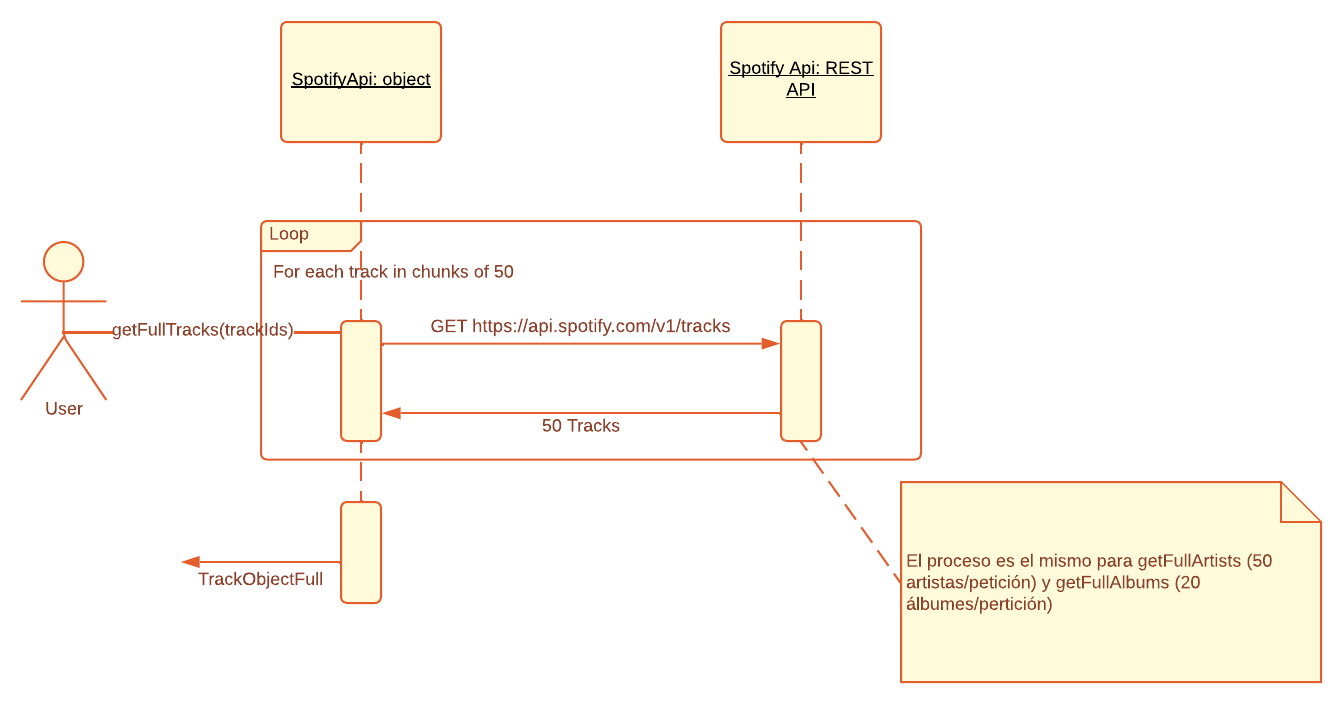
\includegraphics{img/C/spotify_data_fetch.png}
    \caption{Obtención de datos de Spotify}
    \label{fig:C:spotify_fetch}
\end{figure}

La figura \ref{fig:C:ludwig_fetch} explica como se analizan las canciones de Spotify teniendo en cuenta que cada canción analizada se persiste en una base de datos para reducir el tiempo de análisis. 



\begin{figure}
    \centering
    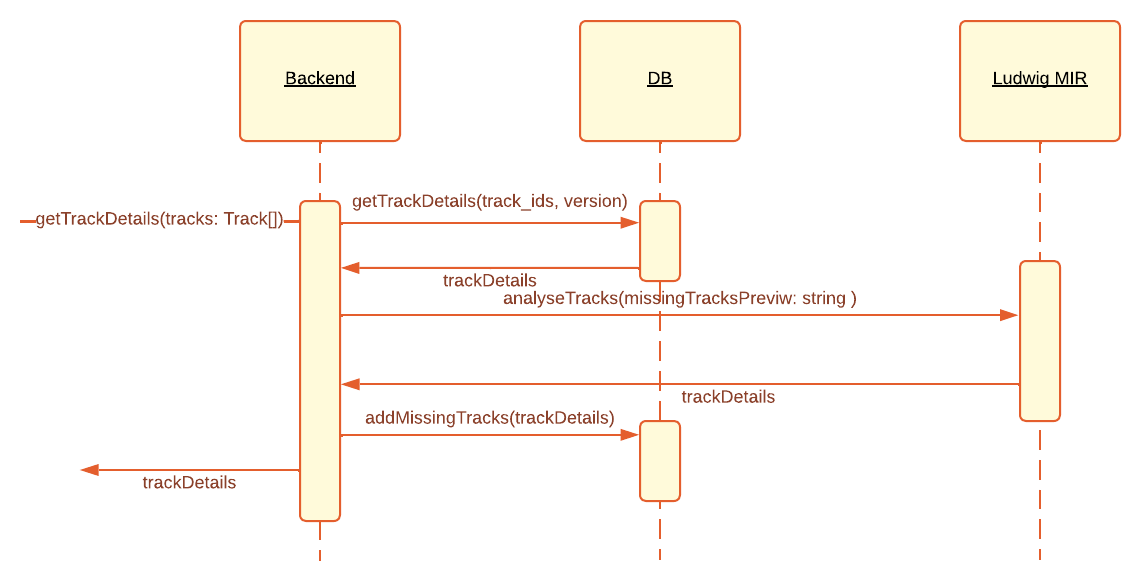
\includegraphics[]{img/C/ludwig_data_fetch.png}
    \caption{Obtención de datos de Ludwig MIR}
    \label{fig:C:ludwig_fetch}
\end{figure}

La figura \ref{fig:C:track_fetch}, al igual que las figuras \ref{fig:C:album_fetch} y \ref{fig:C:artist_fetch} hace referencia a como obtener datos homogéneos a partir de la API de Spotify, LastFM y el Backend Nextjs\footnote{El backend NextJS a su vez se comunica con el Backend de recuperación de información musical y la base de datos}.

La obtención de canciones homogéneas se puede resumir en los siguientes pasos:
    
\begin{enumerate}
    \item  Carga los elementos de la caché a partir de su ID y calcula los elementos que no están cacheados.
    \item Pide a Spotify mediante el proceso de la figura \ref{fig:C:spotify_fetch} las canciones completas. 
    \item Pide al servidor web Ludwig que analice todas las canciones. Este paso se inicia en este punto porque es paso más largo.
    \item Realiza el proceso de la fachada con los artistas Fig.\ref{fig:C:artist_fetch} y álbumes Fig.\ref{fig:C:album_fetch} con todos los álbumes y artistas que ha devuelto la API de Spotify.
    \item Una vez acabados los pasos anteriores, realiza una operación de $join$ que une cada canción con su álbum y artista asociado, esta operación además persiste los datos en la caché local.
    \item Devuelve las canciones homogéneas. Las canciones será actualizadas por referencia una vez se obtengan los resultados del análisis. 
\end{enumerate}


\begin{figure}
    \centering
    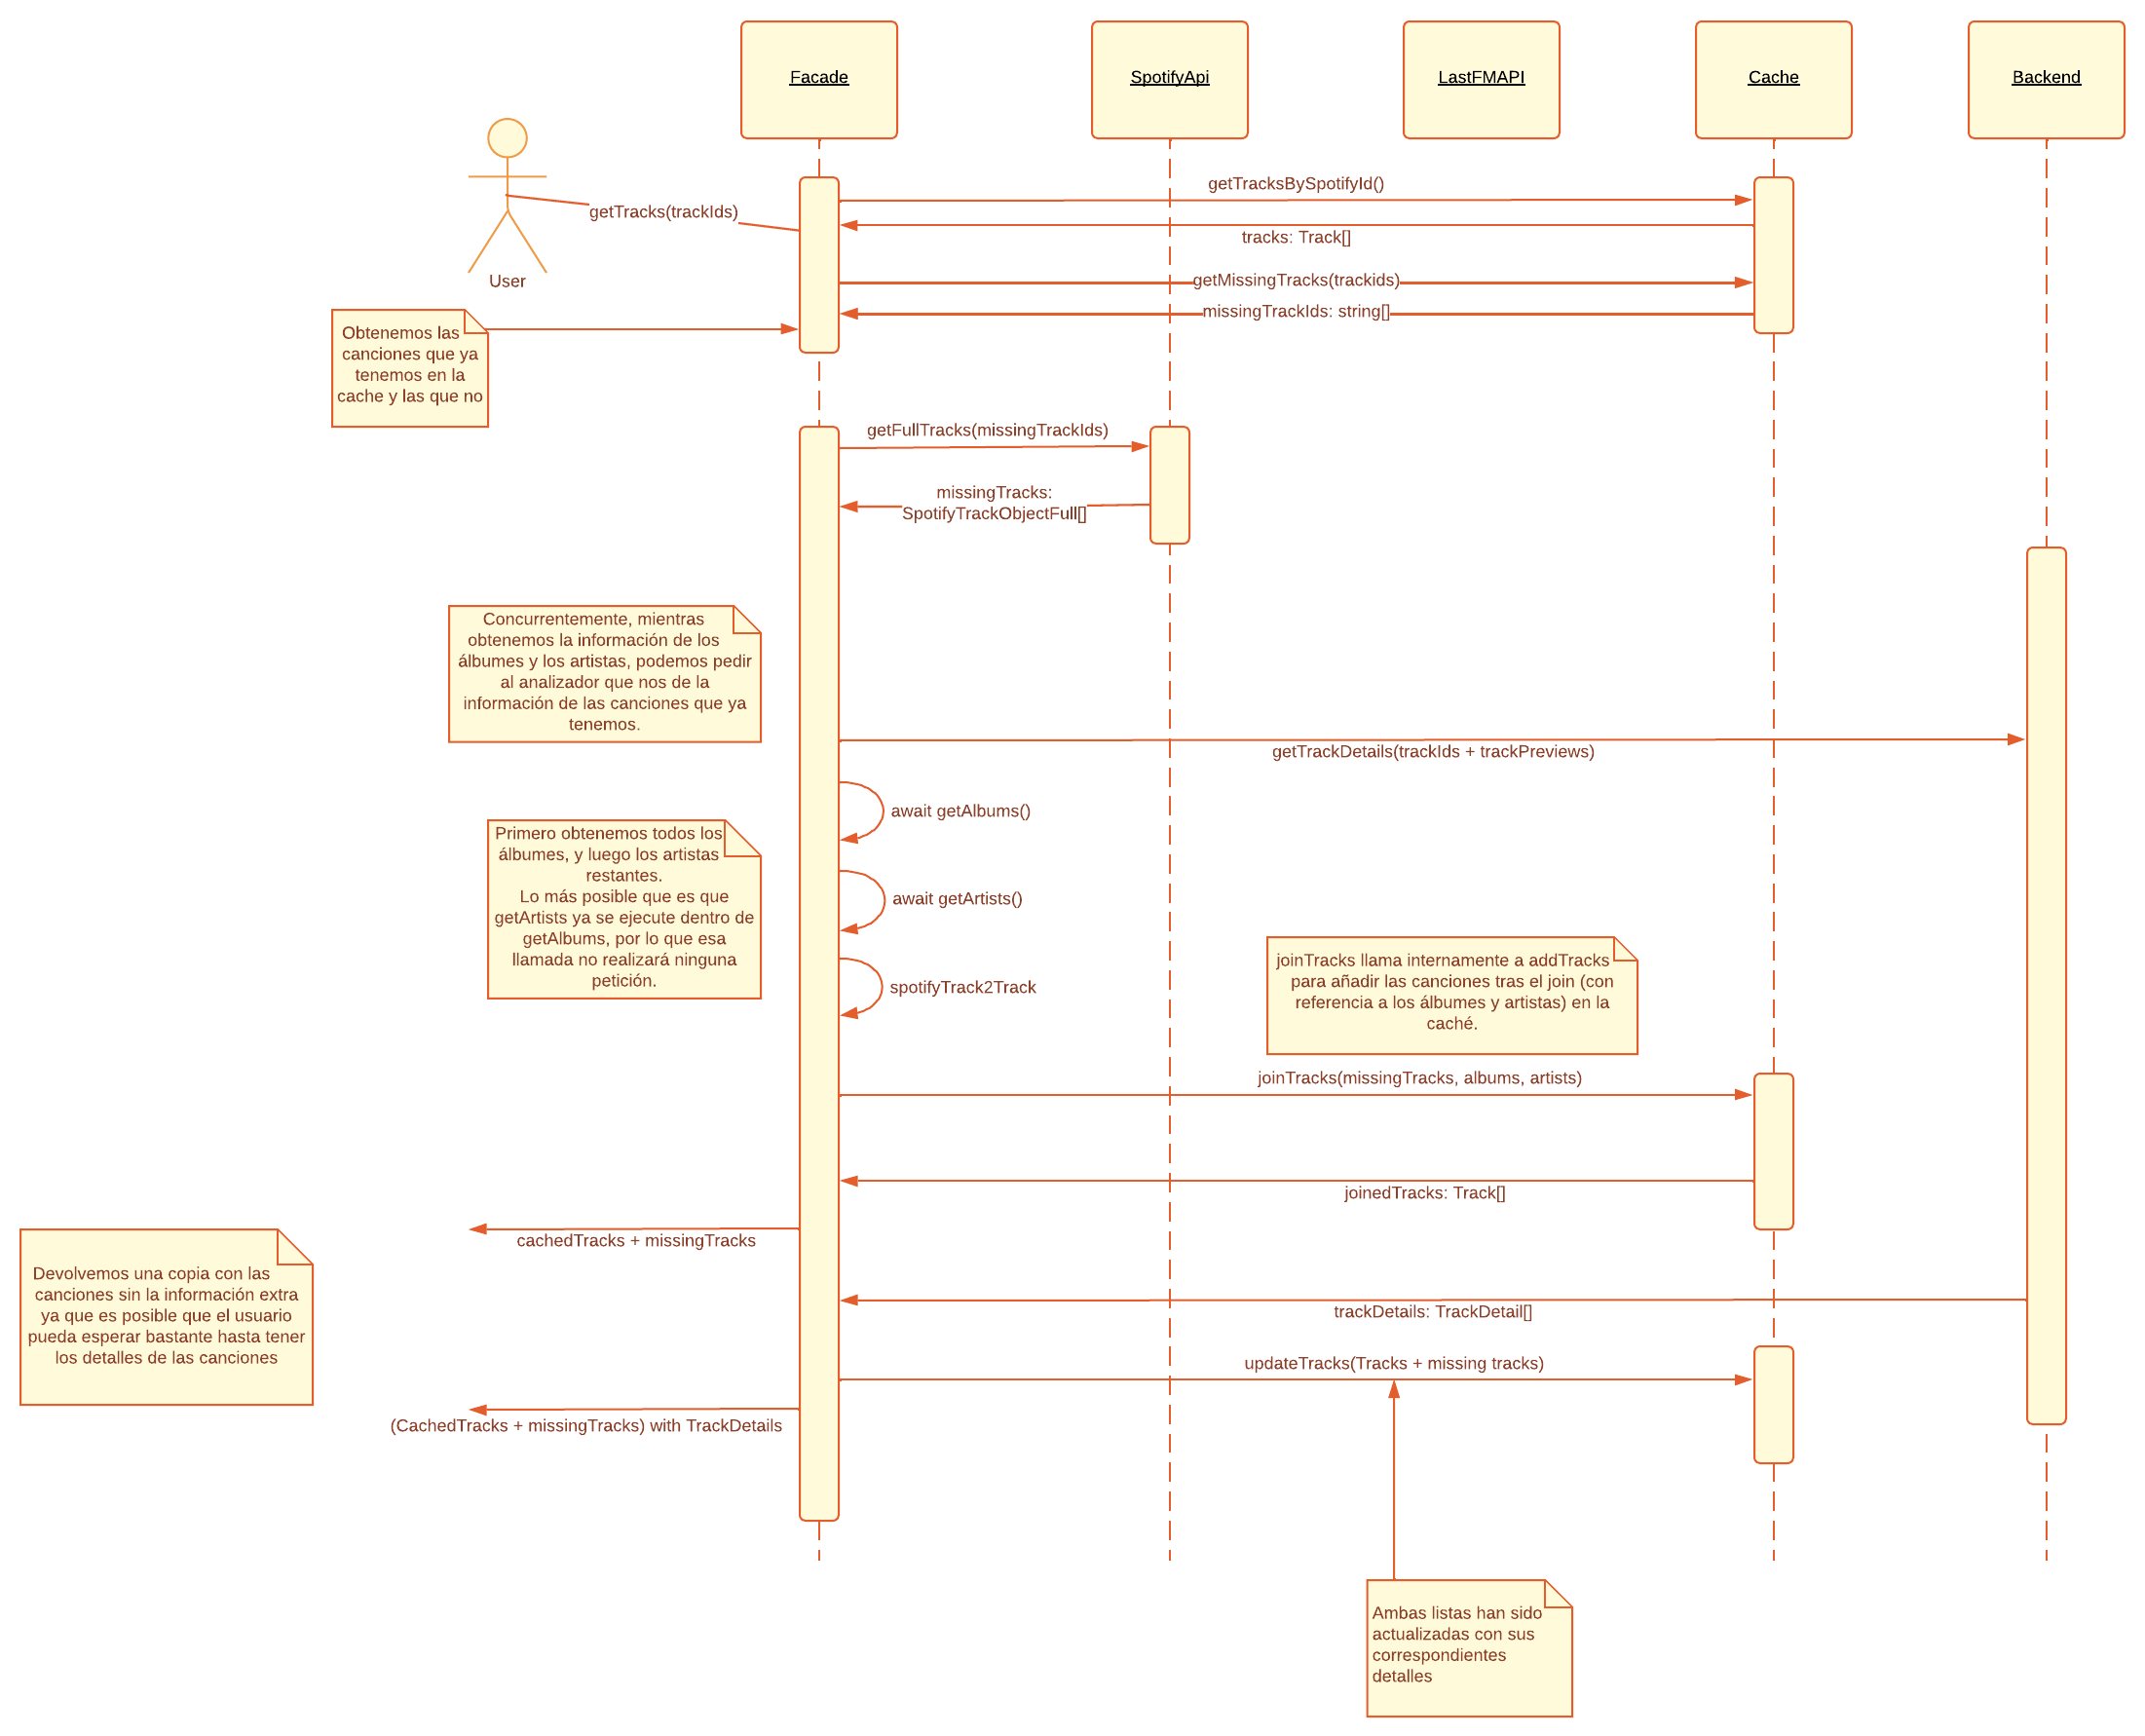
\includegraphics[angle=90]{img/C/track_fetch.png}
    \caption{Obtención de canciones de Spotify}
    \label{fig:C:track_fetch}
\end{figure}


\begin{figure}
    \centering
    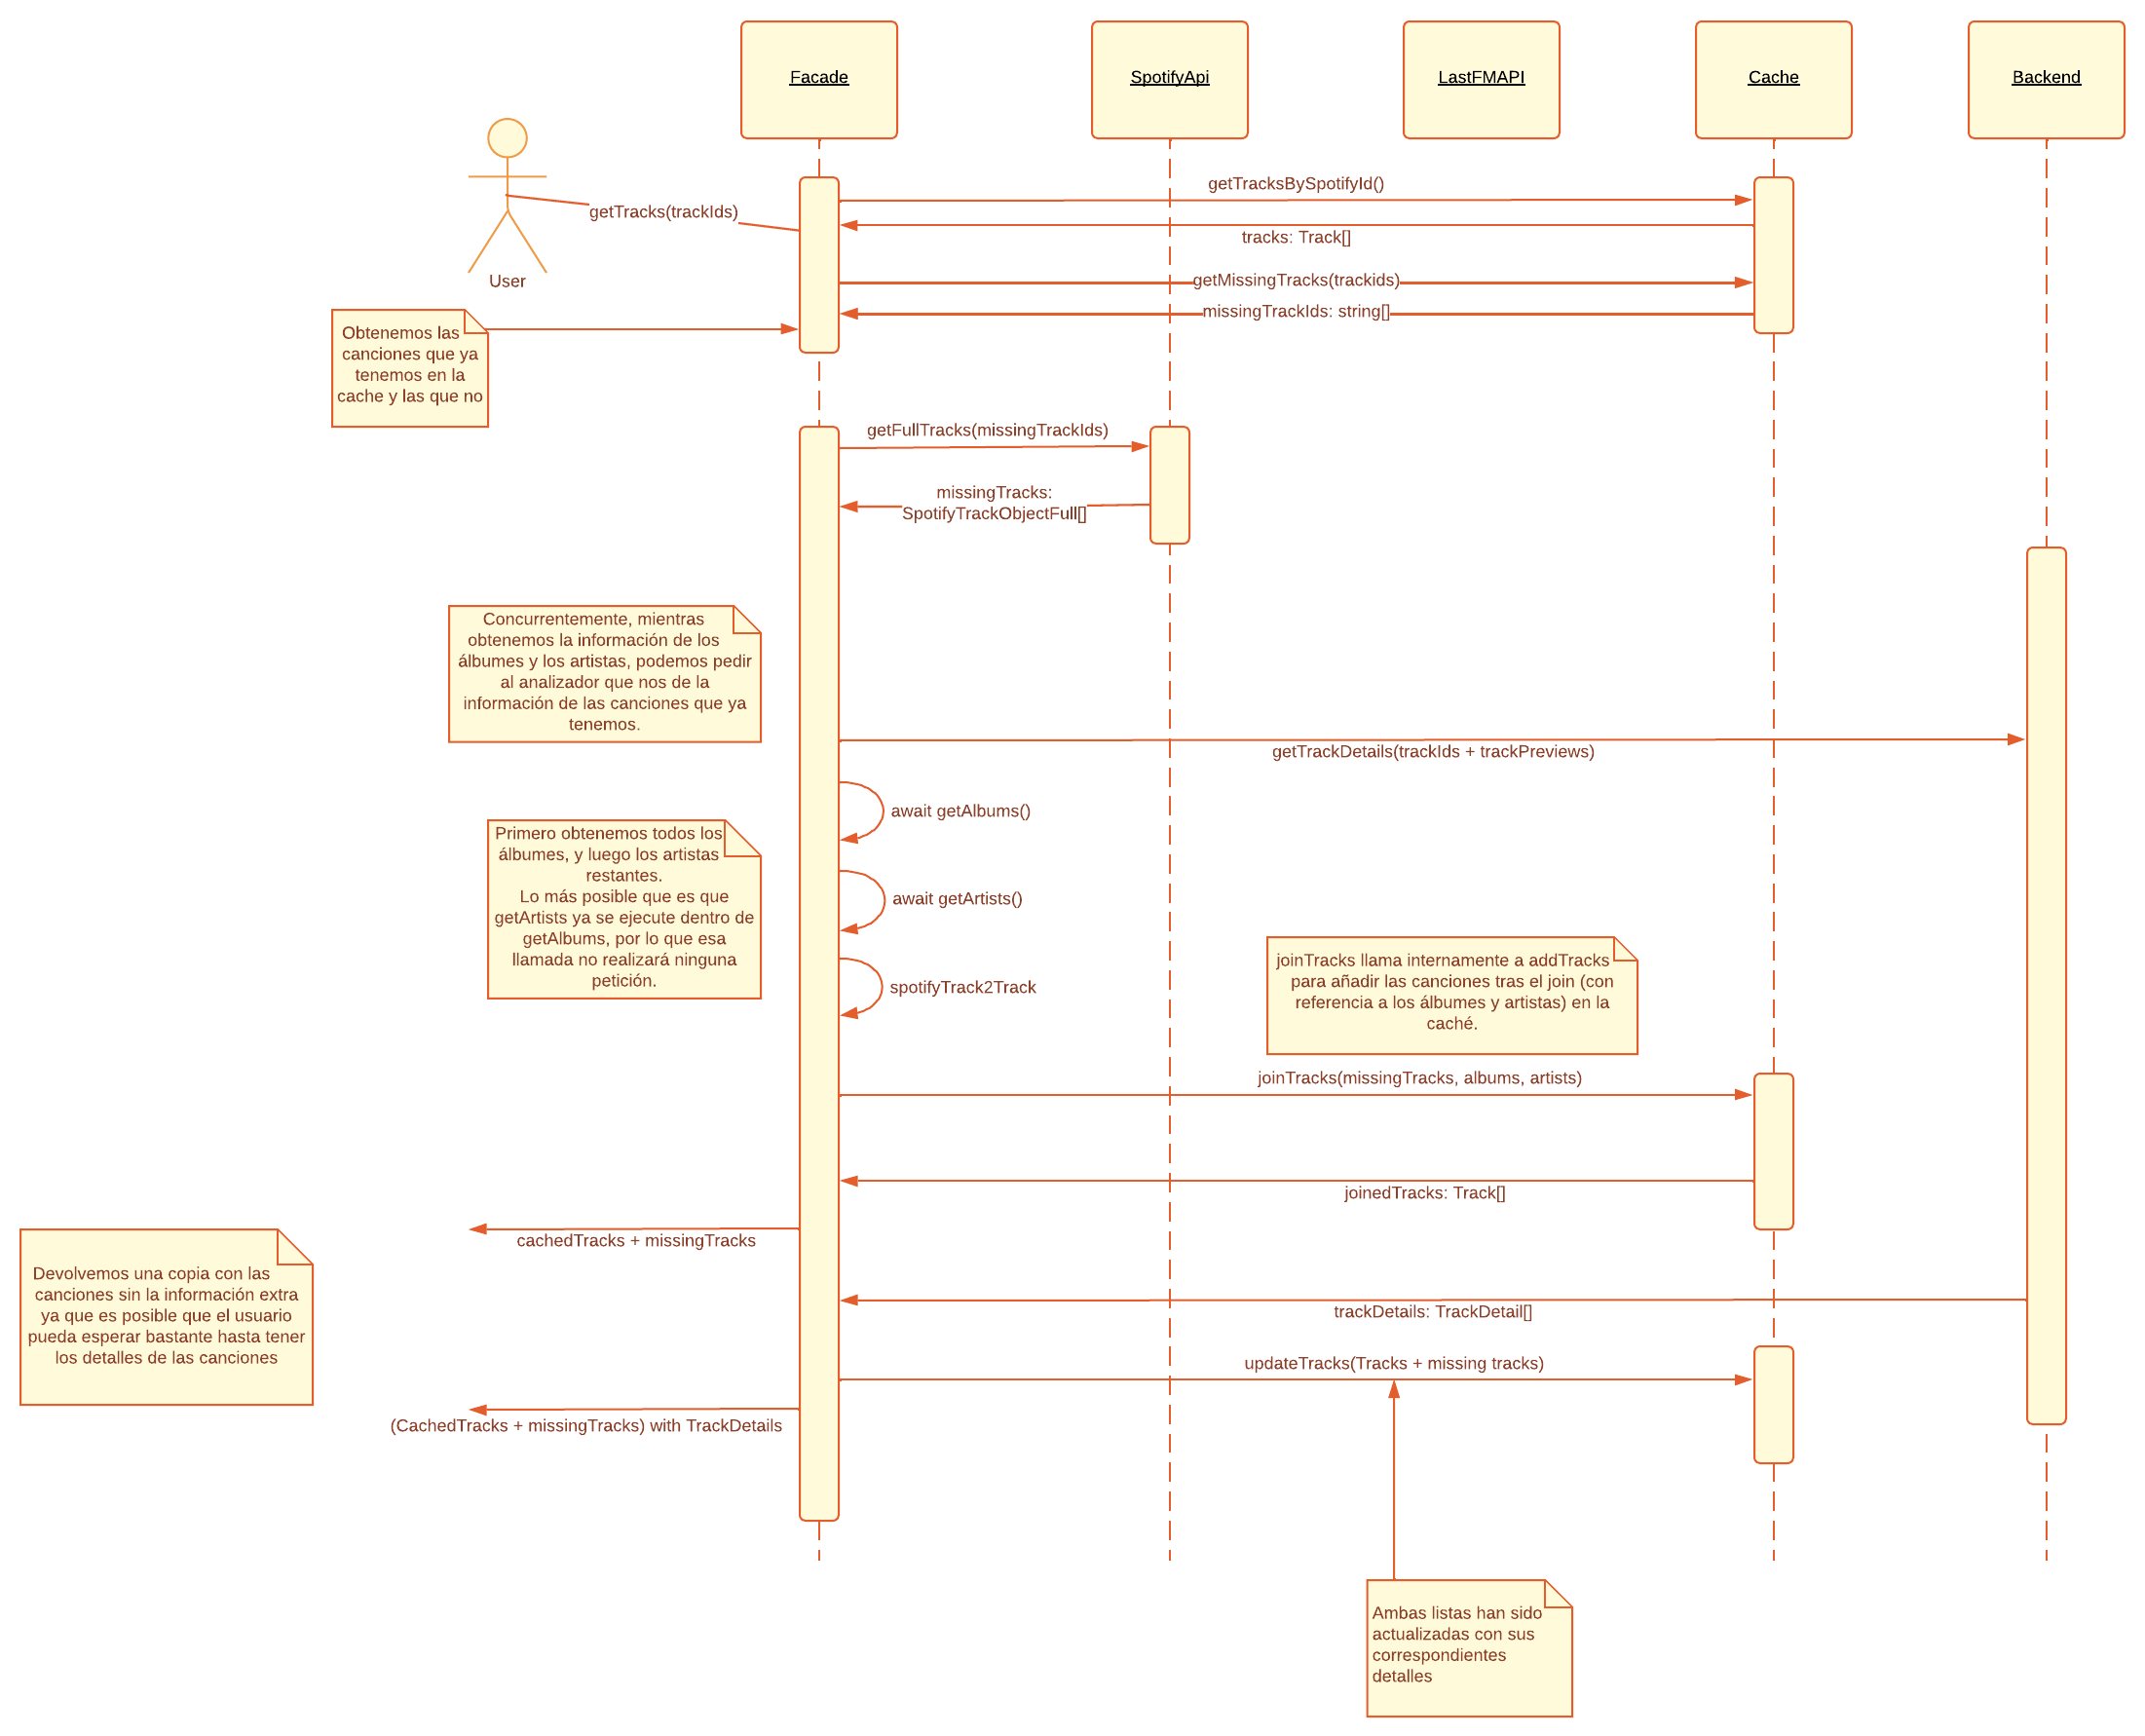
\includegraphics[angle=90]{img/C/track_fetch.png}
    \caption{Obtención de álbumes de Spotify}
    \label{fig:C:album_fetch}
\end{figure}

\begin{figure}
    \centering
    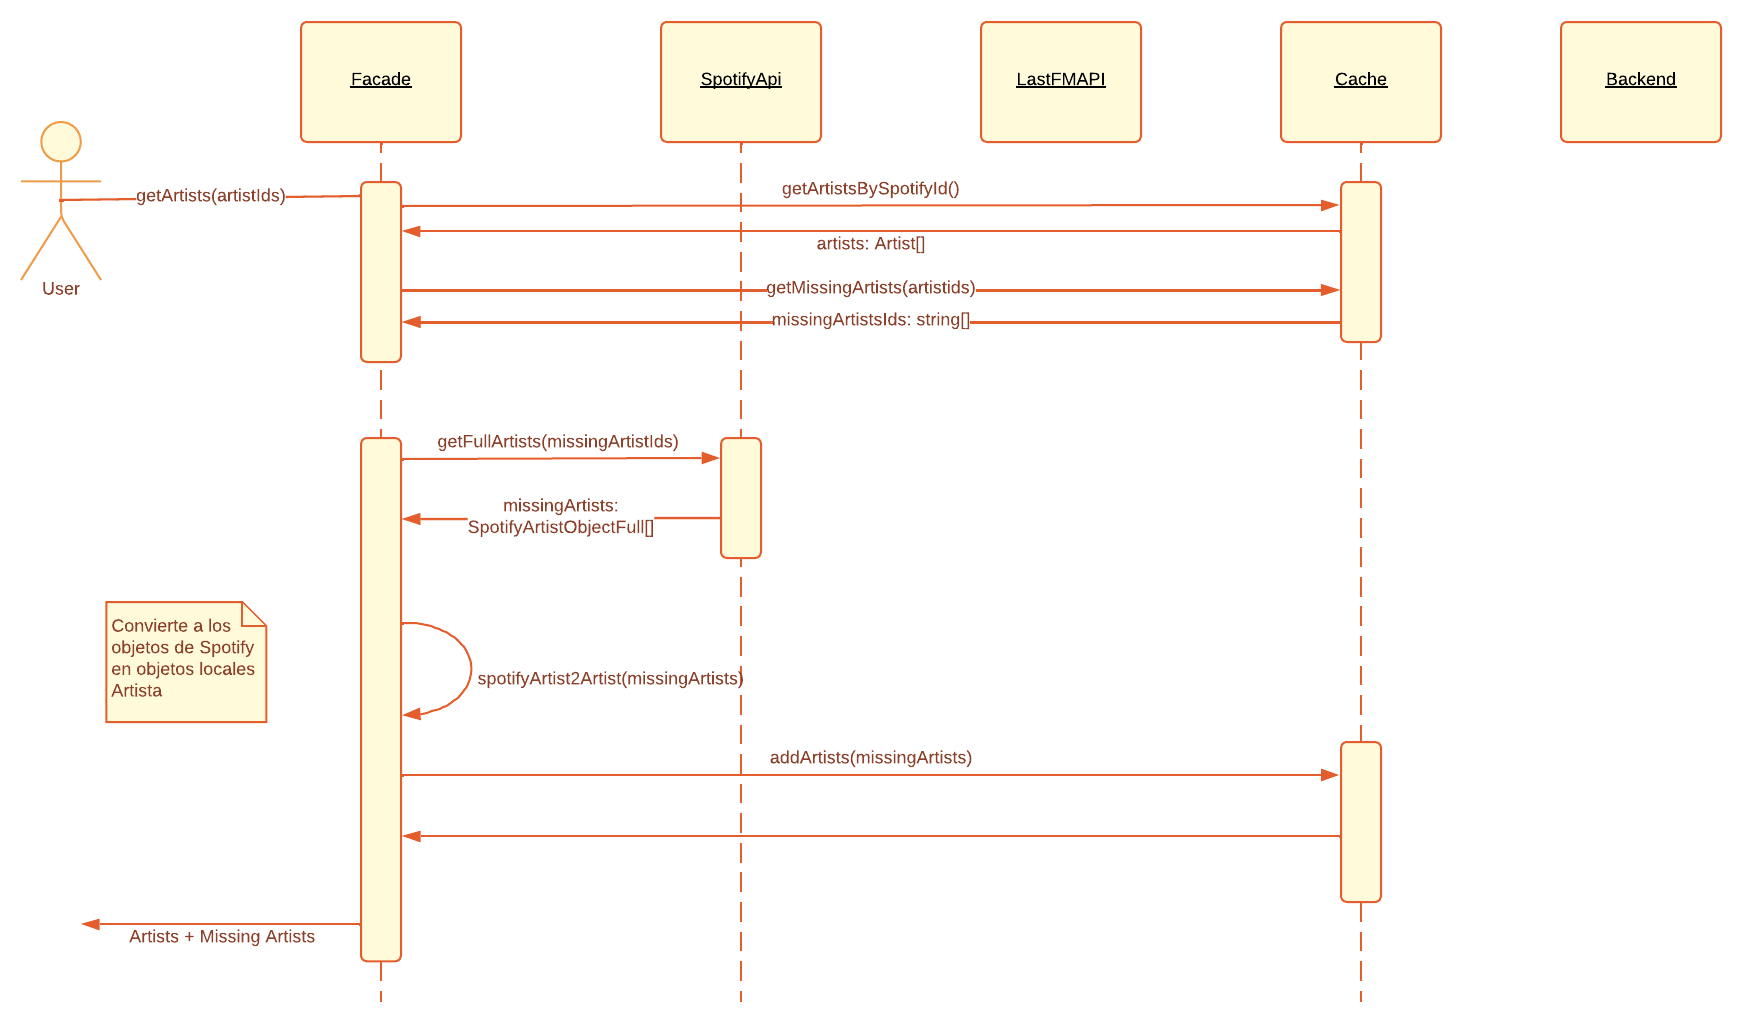
\includegraphics[angle=90]{img/C/artist_fetch.png}
    \caption{Obtención de artistas de Spotify}
    \label{fig:C:artist_fetch}
\end{figure}

\clearpage

\section{Diseño Arquitectónico}

Este apartado concreta los elementos más relevantes sobre la arquitectura del proyecto. 

\subsection{Motor de Inferencia}

Para gestionar el elevado número de clasificadores de subgéneros, se ha diseñado el motor de inferencia recursivo de la figura \ref{fig:C:IE} aplicando el patrón de diseño Composite \cite{C:Composit36:online}. Este motor se configura mediante un fichero .json, donde se recogen los géneros y subgéneros de cada uno de los clasificadores, así como la ruta del modelo en formato ONNX. 

El motor de inferencia agrupa los distintos MFCCs de 3s de duración en un único lote, minimizando el tiempo de inferencia. Cada lote agrupa las $Inference Request$\footnote{Peticiones de Inferencia} por su género o subgénero. Por ejemplo, el clasificador de géneros agrupará las peticiones de inferencia en 9 grupos, siendo cada grupo un género musical. El nodo pasará cada uno de los lotes a su correspondiente Nodo Hijo, que etiquetará los subgéneros de cada canción actualizando el campo de la petición por referencia.


\begin{figure}
    \centering
    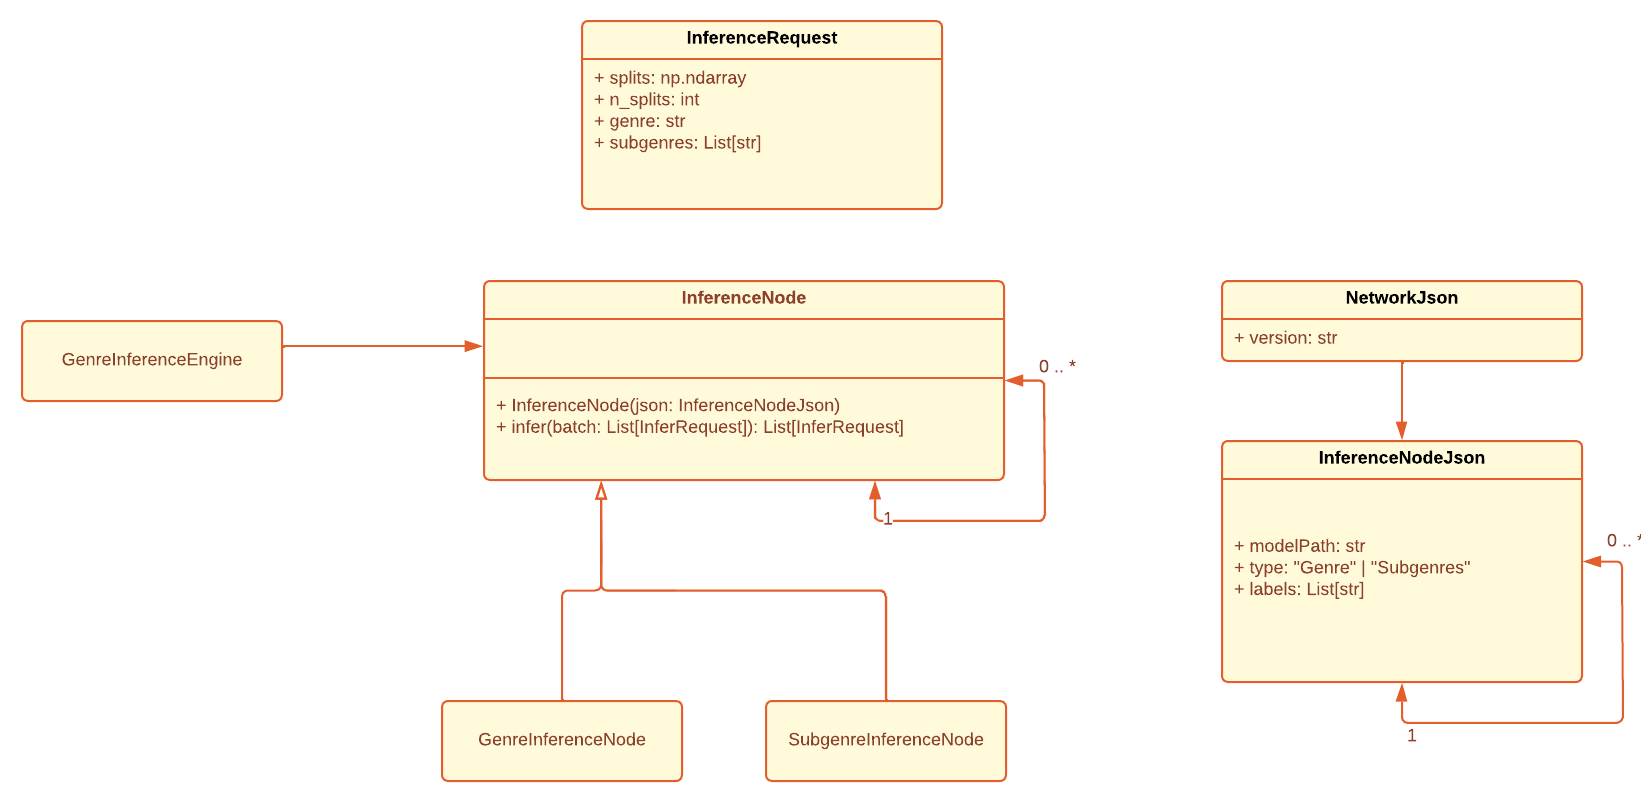
\includegraphics{img/C/IE.png}
    \caption{Motor de Inferencia}
    \label{fig:C:IE}
\end{figure}


\subsection{Patrón MVP} \label{modelo_vista_presentador}

El patrón Modelo Vista Presentador \cite{C:MVP:enwiki:1054194939} es un patrón de software utilizado para construir interfaces.\\
En este patrón nos encontramos tres componentes:
\begin{enumerate}
    \item \textbf{Modelo}: Formado por los datos que va a utilizar el Presentador.
    \item \textbf{Vista}: La interfaz pasiva que muestra los datos procesados por el Presentador.
    \item \textbf{Presentador}: Es el elemento que interactúa entre el Modelo y la Vista, permite obtener los datos de la vista (entrada de usuario) y del modelo, procesarlos y modificar la vista en función a los cambios. 
\end{enumerate}

En este proyecto, el Modelo es la caché de datos y los distintos clientes REST, la vista es el Javascript y HTML generado por ReactJs y el presentador son los Componentes y Hooks de ReactJS escritos en TSX y TS respectivamente. 

\subsection{Fachada de Datos}\label{C:fachada_datos}

Para gestionar el flujo de datos especificado en los diagramas de secuencia  del aparatado \ref{C:obtencion_datos_flow}, se ha detallado un diagrama de clases en la figura \ref{fig:C:facade} con todos los métodos necesarios que detallan las distintas interfaces de los clientes REST, caché local, etc.

En este caso, todos los clientes REST implementan una interfaz común para tratar los errores HTTP, independientemente del cliente HTTP utilizado. 

\begin{figure}
    \centering
    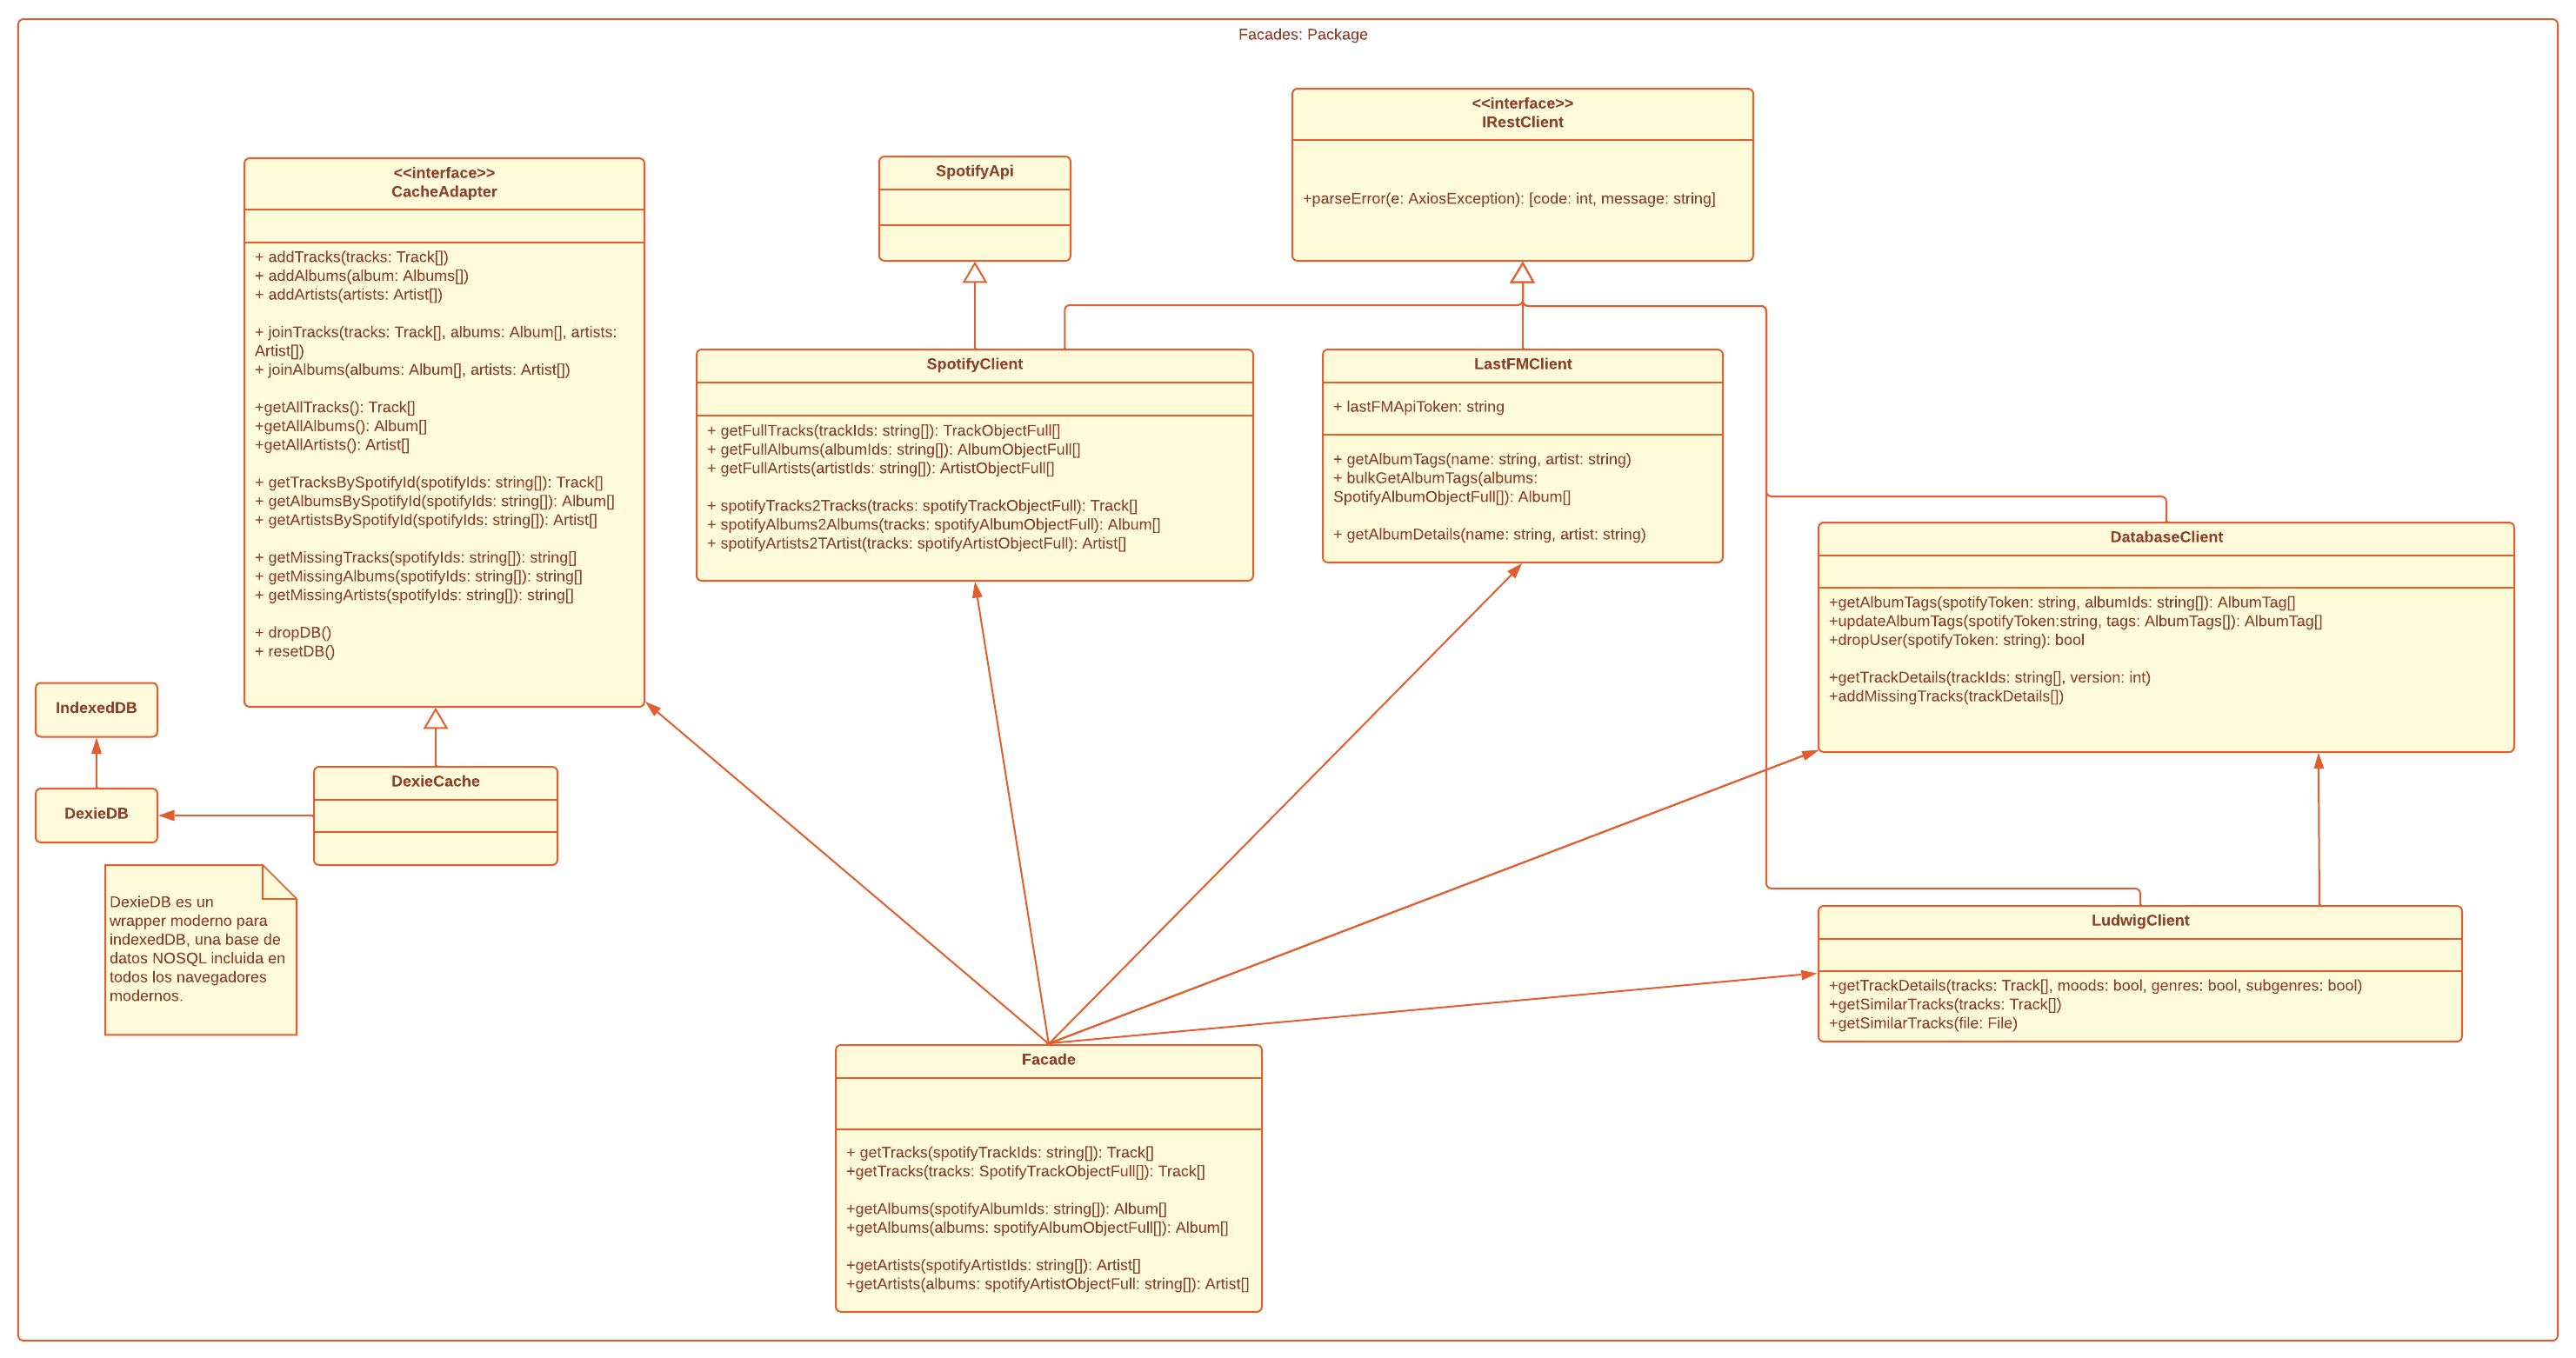
\includegraphics[angle=90,width=\linewidth,height=\textheight,keepaspectratio]{img/C/facade.png}
    \caption{Fachada de Datos}
    \label{fig:C:facade}
\end{figure}


\subsection{Modelo Serverless}

El modelo serverless es un tipo de arquitectura de Cloud Computing que permiten ejecutar y escalar un servicio web sin necesidad de gestionar las máquinas físicas o servidores. 
En el caso de este proyecto, se han usado dos paradigmas serverless: Functions as a Service (FaaS) y Containers as a Service (CaaS). 

Functions as a Service es un paradigma que permite ejecutar funciones sueltas como si fuesen un endpoint de una API. En este caso, por cada petición se levanta un pequeño servicio en los servidores del proveedor cloud, que gestionará la petición HTTP. Una vez se termine la petición, se elimina la instancia de la función.
Podemos disfrutar de este paradigma si desplegamos la platforma con un proveedor cloud compatible, como Netlify o Vercel. 

Containers as a Service es un paradigma que permite instanciar APIs almacenadas en un contenedor de manera similar a FaaS. En este caso, el proveedor cloud permite tener una pool de contenedores, y esta se gestiona automáticamente dependiendo de las necesidades del servicio.
Los dos servidores se han desplegado siguiendo este paradigma. 

Ambos paradigmas permiten escalar de una forma muy directa los distintos servicios, ya que se pueden desplegar tantos servicios como peticiones y en los servidores más cercanos al usuario. El principal inconveniente de estos paradigmas es el tiempo de arranque, ya que si la función o el contenedor tiene un gran número de dependencias, el arranque puede durar varios segundos para gestionar una petición HTTP pequeña que apenas requiere unos pocos cientos de milisegundos de tiempo de ejecución.


\subsection{Guía de Estilo}
Este apartado contiene una guía de estilo con los colores y tamaños de letra utilizados en el frontend. La guía ha sido generada mediante la herramienta Catalog \cite{Catalog1:online}

\label{anexo:guia_estilo}
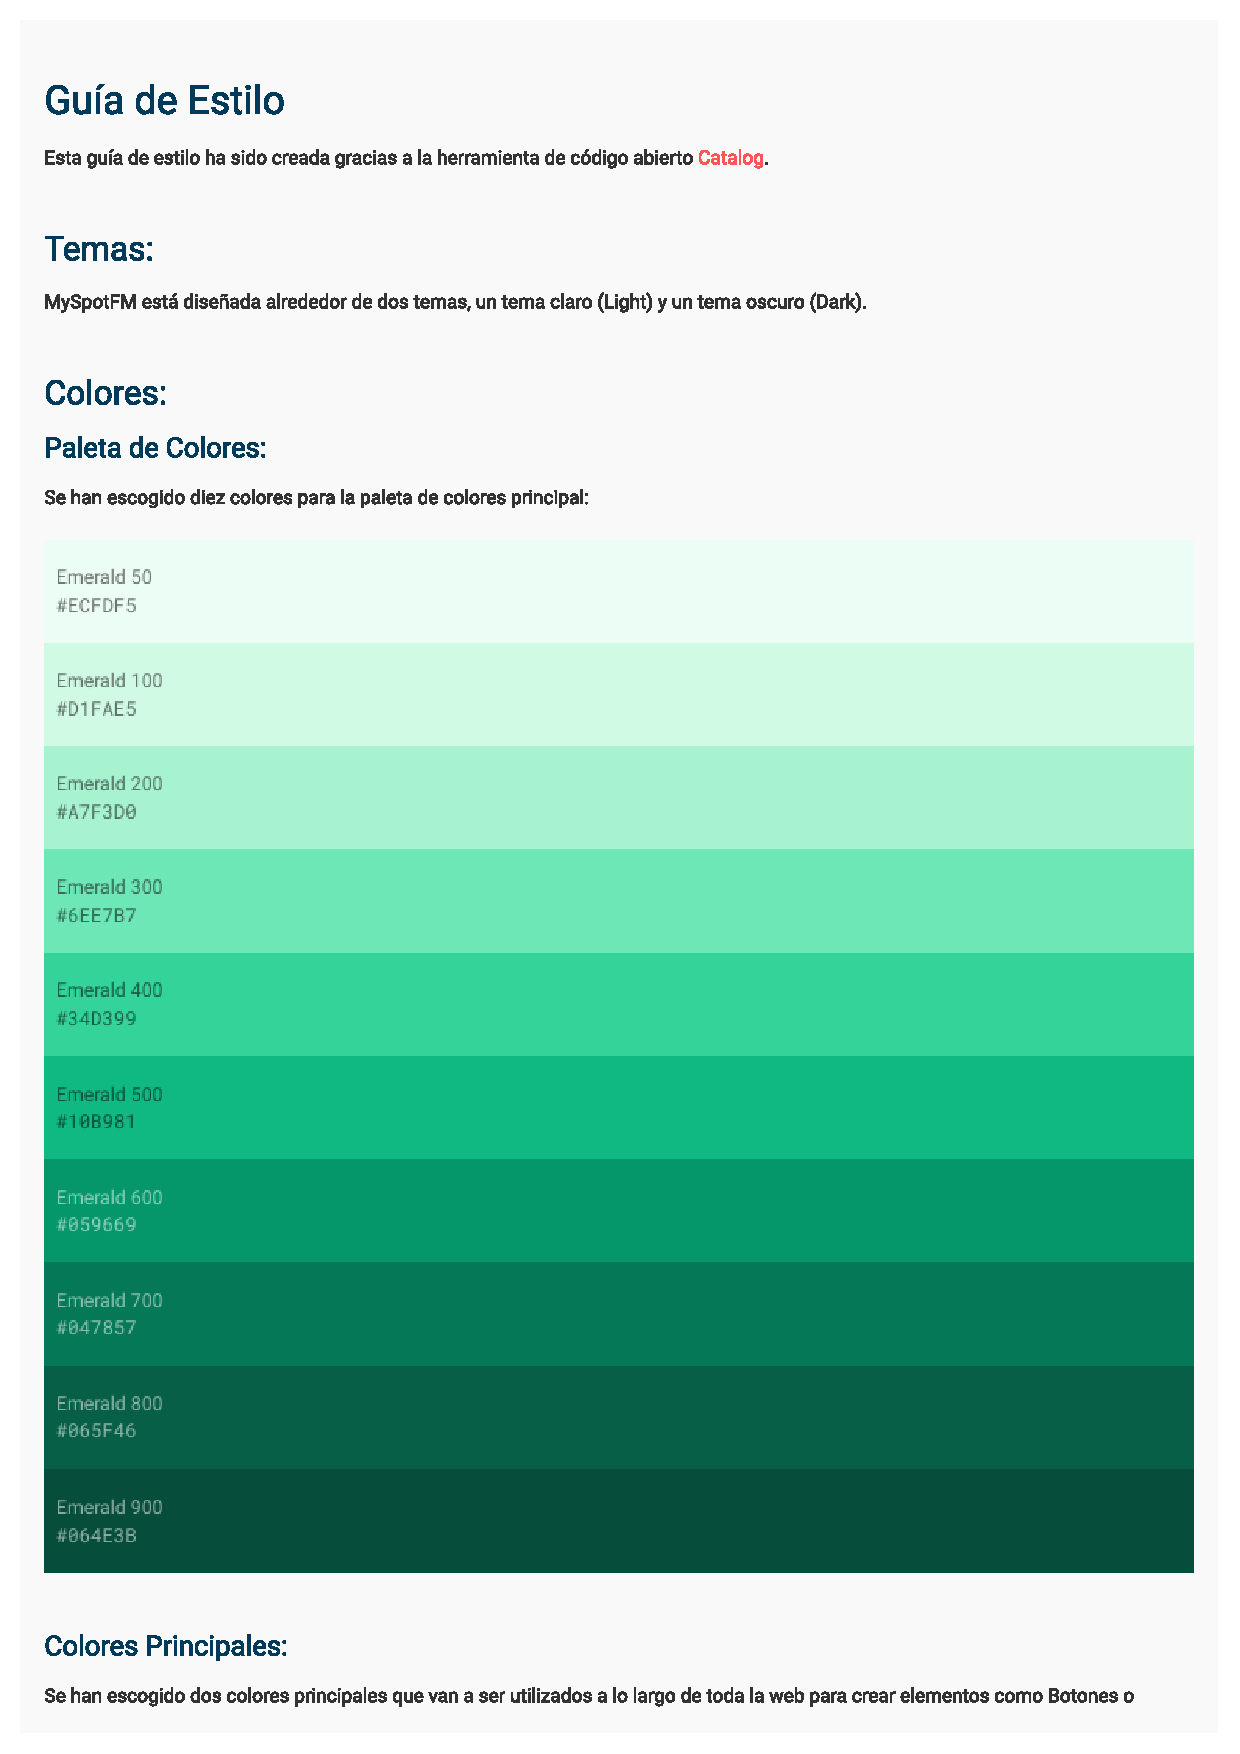
\includepdf[pages=-]{img/C/StyleGuideExport.pdf}
\clearpage
\section{Diseño de Redes Neuronales}

Este apartado detalla la arquitectura de las redes neuronales convolucionales que se han utilizado a lo largo del proyecto. Todas la redes tienen como entrada un tensor con dimensión $N\times130\times32$, correspondiente a un bloque de $N$ MFCCs de 3 segundos de duración.

\subsection{CNN: Clasificador de Géneros}
El clasificador de géneros está formado por 2 redes neuronales. Por un lado se ha utilizado la arquitectura EfficientNetB0 \cite{C:efficentnet} como base del clasificador. Esta arquitectura requiere que la entrada tenga 3 canales, ya que está pensada para el tratamiento de imágenes RGB, por lo que es necesario añadir 2 canales a nuestros MFCCs. Para ello se ha usado una capa convolucional como entrada de la red, que permite expandir la entrada con otras 2 copias.
A la salida de la red EfficientNetB0, se ha añadido una capa GlobalAveragePooling (GAP), que normaliza la salida de la red al realizar una operación de pooling en cada dimensión, reduciendo la dimensión de la salida de forma similar a una capa Flatten. Por último se añaden dos capas densas, la capa de salida con 9 neuronas equivalentes al número de clases, y una capa intermedia entre GAP y la capa de salida, con activación Softmax. Esta red se corresponde con la figura \ref{fig:C:cnn_0}, donde dense\_6 es la salida de la red.

\begin{figure}
    \centering
    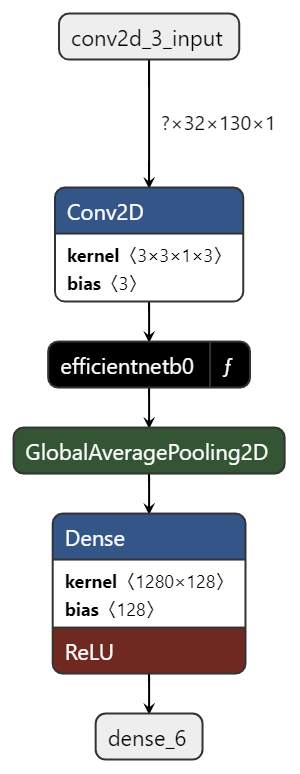
\includegraphics[width=0.33\textwidth,height=\textheight,keepaspectratio]{img/C/cnn_genre_0.png}
    \caption{Arquitectura del Clasificador de Géneros}
    \label{fig:C:cnn_0}
\end{figure}

\subsection{CNN: Clasificador de Subgéneros}\label{c:clas_subg}

El clasificador de subgéneros es una red neuronal convolucional convencional \ref{fig:C:cnn_subgéneros}, formada por bloques convolucionales formados por:

\begin{itemize}
    \item Operación de convolución.
    \item Operación de normalización.
    \item Operación de Pooling.
    \item Segunda operación de normalización.
\end{itemize}

En este caso, la salida de la red es una capa densa con $N$ neuronas, siendo $N$ el número de subgéneros que es capaz de detectar dicha capa. Esta capa tiene como función de activación la función Sigmoide. 

\begin{figure}
    \centering
    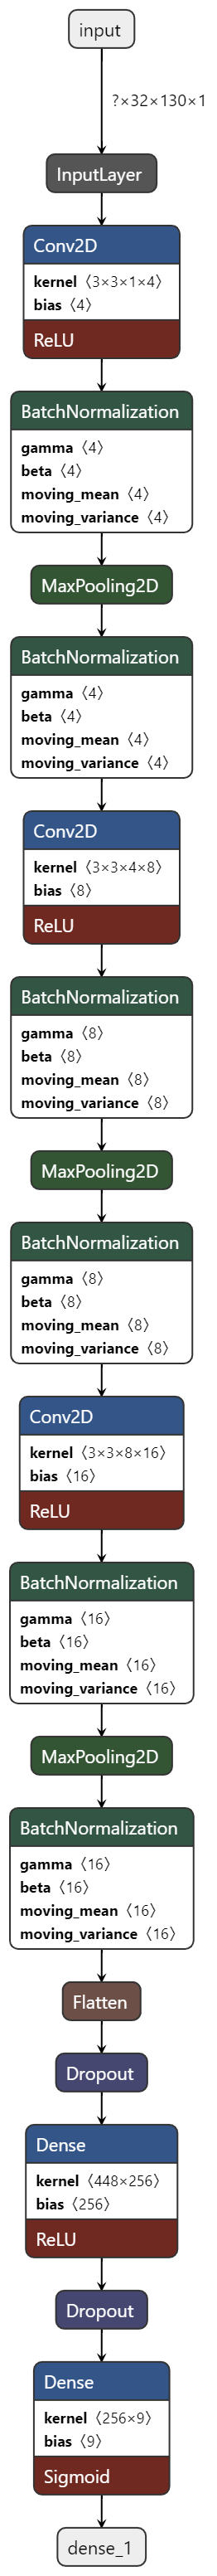
\includegraphics[width=\textwidth,height=\textheight,keepaspectratio]{img/C/cnn_sub.png}
    \caption{Arquitectura del Clasificador de Subgéneros}
    \label{fig:C:cnn_subgéneros}
\end{figure}


\subsection{Ova de CNN: Clasificador de Estados de Ánimo}

El clasificador de estados de ánimo \ref{fig:C:ova} es una OVA de 7 CNNs binarias activadas mediante una Sigmoide. Cada una de las CNNs tiene una arquitectura muy similar a \ref{c:clas_subg}.\\
La salida de la red es una capa de concatenación que junta todas las salidas en un único tensor.

\begin{figure}
    \centering
    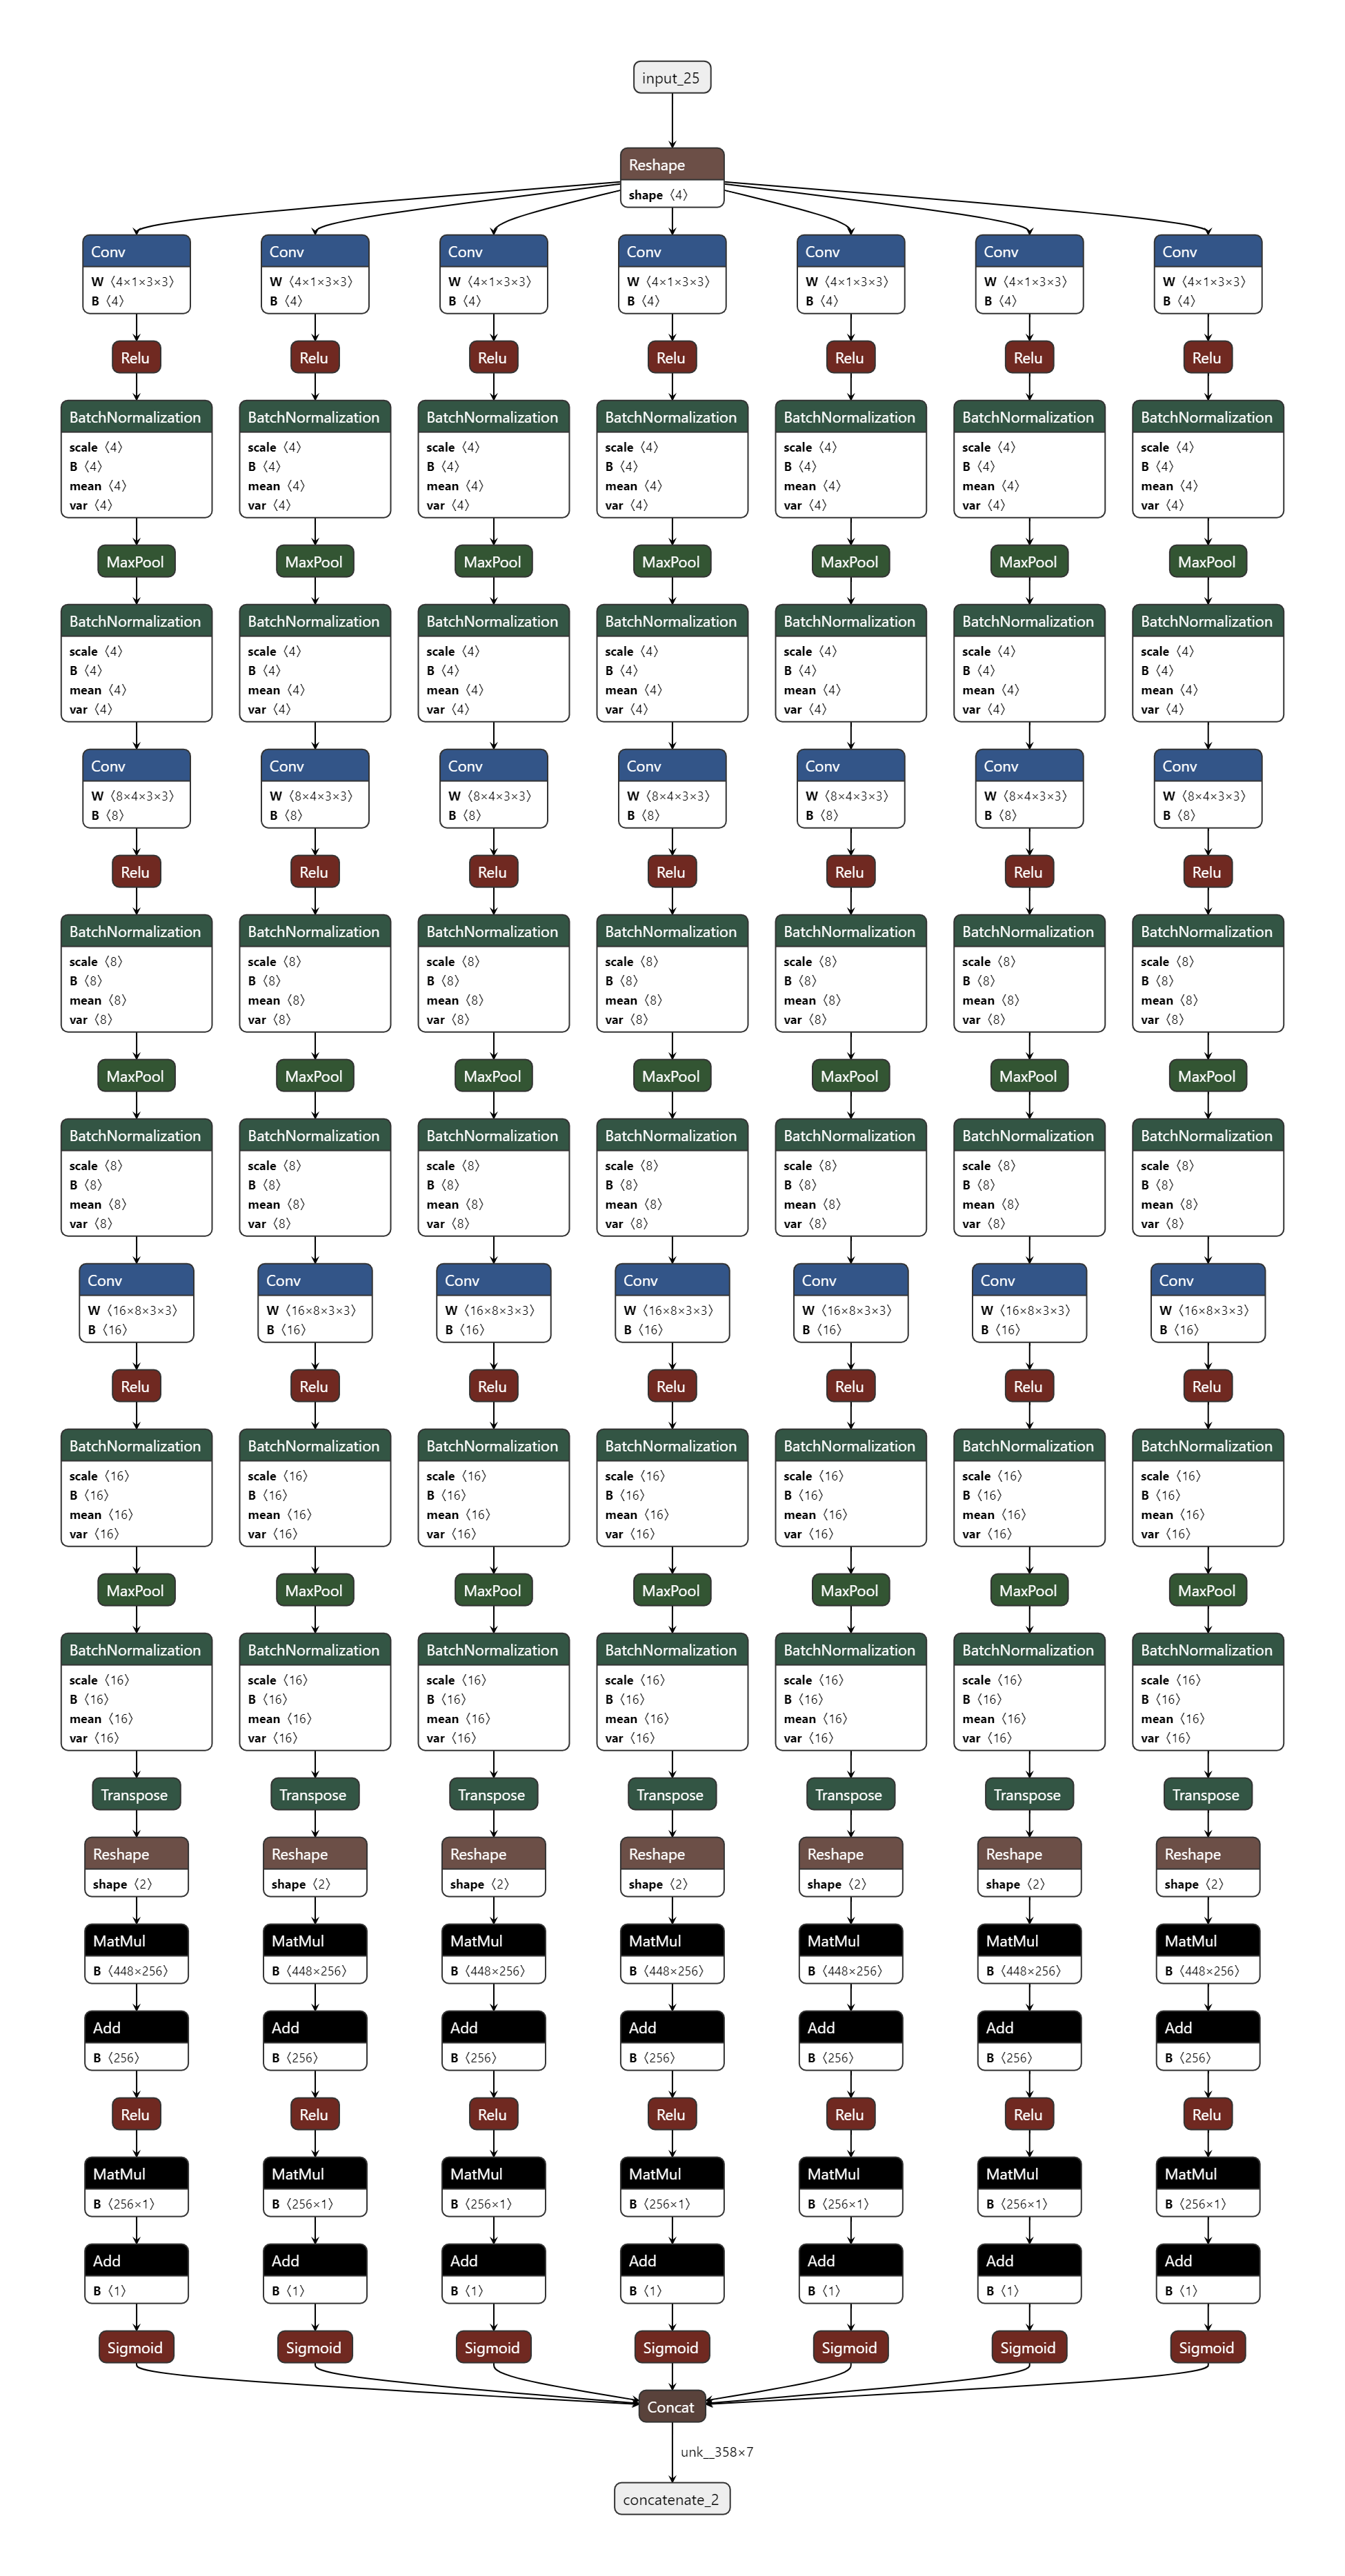
\includegraphics[width=\textwidth,height=\textheight,keepaspectratio]{img/C/cnn_moods_ova.png}
    \caption{Arquitectura del Clasificador de Estados de Ánimo}
    \label{fig:C:ova}
\end{figure}

